%% Copernicus Publications Manuscript Preparation Template for LaTeX Submissions
%% ---------------------------------
%% This template should be used for copernicus.cls
%% The class file and some style files are bundled in the Copernicus Latex Package, which can be downloaded from the different journal webpages.
%% For further assistance please contact Copernicus Publications at: production@copernicus.org
%% https://publications.copernicus.org/for_authors/manuscript_preparation.html


%% Please use the following documentclass and journal abbreviations for discussion papers and final revised papers.

%% 2-column papers and discussion papers
\documentclass[os, manuscript]{copernicus}



%% Journal abbreviations (please use the same for discussion papers and final revised papers)


% Advances in Geosciences (adgeo)
% Advances in Radio Science (ars)
% Advances in Science and Research (asr)
% Advances in Statistical Climatology, Meteorology and Oceanography (ascmo)
% Annales Geophysicae (angeo)
% Archives Animal Breeding (aab)
% ASTRA Proceedings (ap)
% Atmospheric Chemistry and Physics (acp)
% Atmospheric Measurement Techniques (amt)
% Biogeosciences (bg)
% Climate of the Past (cp)
% DEUQUA Special Publications (deuquasp)
% Drinking Water Engineering and Science (dwes)
% Earth Surface Dynamics (esurf)
% Earth System Dynamics (esd)
% Earth System Science Data (essd)
% E&G Quaternary Science Journal (egqsj)
% Fossil Record (fr)
% Geochronology (gchron)
% Geographica Helvetica (gh)
% Geoscience Communication (gc)
% Geoscientific Instrumentation, Methods and Data Systems (gi)
% Geoscientific Model Development (gmd)
% History of Geo- and Space Sciences (hgss)
% Hydrology and Earth System Sciences (hess)
% Journal of Micropalaeontology (jm)
% Journal of Sensors and Sensor Systems (jsss)
% Mechanical Sciences (ms)
% Natural Hazards and Earth System Sciences (nhess)
% Nonlinear Processes in Geophysics (npg)
% Ocean Science (os)
% Primate Biology (pb)
% Proceedings of the International Association of Hydrological Sciences (piahs)
% Scientific Drilling (sd)
% SOIL (soil)
% Solid Earth (se)
% The Cryosphere (tc)
% Weather and Climate Dynamics (wcd)
% Web Ecology (we)
% Wind Energy Science (wes)


%% \usepackage commands included in the copernicus.cls:
%\usepackage[german, english]{babel}
%\usepackage{tabularx}
%\usepackage{cancel}
%\usepackage{multirow}
%\usepackage{supertabular}
%\usepackage{algorithmic}
%\usepackage{algorithm}
%\usepackage{amsthm}
%\usepackage{float}
%\usepackage{subfig}
%\usepackage{rotating}


\begin{document}

\title{Barotropic vorticity balance of the North Atlantic subpolar gyre in an eddy-resolving model}

\Author[1]{Mathieu}{Le Corre}
\Author[1]{Jonathan}{Gula}
\Author[1]{Anne-Marie}{Tréguier}

\affil[1]{Univ. Brest, CNRS, IRD, Ifremer, Laboratoire d'Oc\'eanographie Physique et Spatiale (LOPS), IUEM, Brest, France}


\correspondence{Mathieu Le Corre (mathieu.lecorre@univ-brest.fr)}

\runningtitle{Vorticity balance in the North Atlantic Subpolar Gyre}

\runningauthor{M. Le Corre et al}





\received{}
\pubdiscuss{} %% only important for two-stage journals
\revised{}
\accepted{}
\published{}

%% These dates will be inserted by Copernicus Publications during the typesetting process.


\firstpage{1}

\maketitle



\begin{abstract}
The circulation in the North Atlantic Subpolar gyre is complex and strongly influenced by the topography. The gyre dynamics is traditionally understood as the result of a topographic Sverdrup balance, which corresponds to a first order balance between the planetary vorticity advection, the bottom pressure torque and the wind stress curl. However, these dynamics have been studied mostly with non-eddy-resolving models and a crude representation of the bottom topography. Here we revisit the barotropic vorticity balance of the North Atlantic Subpolar gyre using a high resolution simulation ($\approx$ 2-km) with topography-following vertical coordinates to better represent the mesoscale turbulence and flow-topography interactions. Our findings highlight that, locally, there is a first order balance  between the bottom pressure torque and the nonlinear terms, albeit with a high degree of cancellation between each other. However, balances integrated over different regions of the gyre -- shelf, slope and interior -- still highlight the important role played by nonlinearities and the bottom drag curls. In particular the flat bottom Sverdrup balance cannot describe the dynamics in the interior of the gyre. The main sources of cyclonic vorticity are the non linear terms due to eddies generated along eastern boundary currents and the time-mean nonlinear terms from the Northwest Corner. Our results suggest that a good representation of the mesoscale activity along with a good positioning of the Northwest corner are two important conditions for a better representation of the circulation in the North Atlantic Subpolar Gyre.
\end{abstract}
%\copyrightstatement{TEXT}


\introduction  %% \introduction[modified heading if necessary]
The North Atlantic Subpolar Gyre (SPG) is a key region for the meridional overturning circulation (MOC). There, the North Atlantic surface waters coming from the subtropical gyre are transformed into denser waters that flow southward and form the lower limb of the MOC. The dynamics of the currents in the SPG is a result of strong buoyancy gradients, intense surface buoyancy and wind forcings, and exchanges of waters with the Nordic Seas through overflows. Understanding these complex dynamics is essential to better understand the mechanisms that drive the variability of the MOC. 

 The dynamics of wind-driven oceanic gyres is traditionally understood as the result of two distinct balances for the interior of the gyre and the boundary of the gyre, where currents flow along topography. In the interior, the flow follows a Sverdrup balance, which corresponds to a first order balance between the wind stress curl and a meridional transport in the barotropic (depth-integrated) vorticity balance. This balance has been shown to hold in the interior of subtropical gyres \citep{hughes2001, TDBAJS14, yeager2015, schoonover2016, sonnewald2019, LBST19}. Where the currents interact with the topography, another term becomes first order in the barotropic vorticity balance: the Bottom Pressure Torque (BPT). The BPT includes the impacts of the bottom topography on the barotropic currents, and derives from the interaction of the abyssal geostrophic flow with the sloping bottom bathymetry. Works by \citet{hughes2000,hughes2001, jackson2006, schoonover2016} have demonstrated the prevalence of the BPT in the global barotropic vorticity balance. They have shown in particular that the BPT is the dominant term in western boundary currents, thus demonstrating that bottom friction and viscous effects were not required to close the vorticity budget of the gyres as hypothesized in the classical works of \citet{stommel1948,Munk1950}. 
 The SPG circulation is strongly shaped by the bottom topography. Due to the weak stratification, the currents have a strong barotropic component \citep{vanaken1995,daniault2016,fischer2004}.  They are thus strongly impacted by the steep topography around the gyre. The importance of the bottom topography in driving the SPG dynamics emerged quite early in the works of \citet{luyten1985} and \citet{wunsch1985}. The prevalence of the BPT in the SPG has also been demonstrated by \citet{greatbatch1991,hughes2001, spence2012, yeager2015}. All studies also pointed out a failure of the flat bottom Sverdrup balance in this area. 

The studies putting forward the importance of the BPT in the SPG have been using coarse resolution models. But currents in the SPG are also strongly influenced by eddies, which can modify the mean flow structure \citep{MW08}. Models then require resolutions able to resolve these effects. Eddy-permitting resolutions have been shown to improve the characteristics of the boundary currents of the SPG, including a better position of the currents, narrower lateral extensions and velocity amplitudes closer to observations \citep{treguier2005,danek2019}. The vertical structure of the currents is also improved with a more barotropic structure for the boundary currents around the SPG \citep{marzocchi2015}. These changes, compared to coarser resolution models, allow the inertial effects to become more important and modify the interactions with the topography. Also, at higher resolution, the viscosity is reduced and the bottom topography and inertial effects become prevalent, allowing the flow to better match the observations \citep{spence2012, schoonover2016}. 

Recently, \citet{sonnewald2019} clustered regions dominated by different barotropic vorticity balances using a global $1^{\circ} \times 1^{\circ}$ model. They retrieved the results of a SPG dominated by BPT effects, but also a part of the gyre dominated by Non-Linear (NL) effects, despite the relatively coarse resolution of the model. \citet{yeager2015} compared results from a $1^{\circ}$ resolution model with an eddy-permitting $1/10^{\circ}$ resolution model, and noticed an increase of the amplitude of the NL term by a factor 3 in some locations. However, it did not modify significantly the first order equilibrium between the wind, planetary vorticity and BPT. The impact of the NL term becomes clearer at higher resolution. With a 1/20$^{\circ}$ resolution simulation \citet{wang2017} showed the importance of this term in the dynamics of recirculation gyres such as the Gulf Stream recirculation gyres, the North Western Corner or the recirculation in the Labrador Sea \citep{lavender2000}.

In addition to the horizontal resolution, the representation of the bottom topography has an impact on the structure of the flow. z-level coordinates have the tendency to create too shallow flows compared to partial step coordinates \citep{pacanowski1998}. Terrain following coordinates ( $\sigma$-level) have proven effective in representing boundary currents \citep{schoonover2016,ezer2016}. The z-level types coordinates tend to have too much viscosity and/or diffusivity close to the topography due to the presence of vertical walls. This effect is corrected when increasing the vertical resolution or using partial steps to converge to results obtained with $\sigma$-coordinates \citep{ezer2004}.

The aim of this paper is to investigate the dynamics of the SPG by analysing the barotropic vorticity balance in a truly eddy-resolving $\sigma$-level coordinate model. To our knowledge no study of the SPG dynamics has ever been conducted at this resolution with this kind of vertical coordinate. The switch in vertical coordinate combined with eddy-resolving resolution might help to resolve smaller scale processes and allow a better representation of flow-topography interactions overall. The paper is organised as follows: The simulation setup is presented in section 2. The mean currents characteristics and variability in the simulation are compared to observations in section 3. The barotropic vorticity balance is analyzed for the full SPG in section 4. The balances corresponding to the different parts of the gyre are further described in section 5. To better understand what is hidden inside the non linear term we analyze it more in detail in section 6. Conclusions are presented and discussed in section 7.  

\section{Model and set-up}
To investigate the impact of the topography on the circulation, it is essential to have a good representation of the flow-topography interactions. To do so, we use a terrain-following coordinate model: the Regional Oceanic Modelling System (ROMS, \citet{shchepetkin2009}) in its CROCO (Coastal and Regional Ocean Community) version \citep{debreu2012}. It solves the hydrostatic primitive equations for velocity, temperature and salinity, using a full equation of state for seawater \citep{shchepetkin2009,shchepetkin2011}. 

To achieve a kilometric resolution at a reasonable cost, we use a one way nesting approach by defining two successive horizontal grids with resolutions $\Delta x \approx 6$ km for the parent grid covering the North Atlantic ocean (NATL) and $\Delta x \approx 2$ km for the child grid covering the SPG (POLGYR). The parent North Atlantic domain is identical to the one in \cite{renault2016}. It has 1152 $\times$ 1059 points  with a horizontal resolution of 6---7 km. The child grid has 2000 $\times$ 1600 points and a horizontal resolution of 2 km. It allows the simulation to be truly eddy resolving in most of the area, as the first Rossby deformation radius has trouble exceeding 10-km over most of the region \citep{chelton1998}. The domains are shown in figure \ref{f01}. 

%varies between 10 and 20 km

\begin{figure}[t]
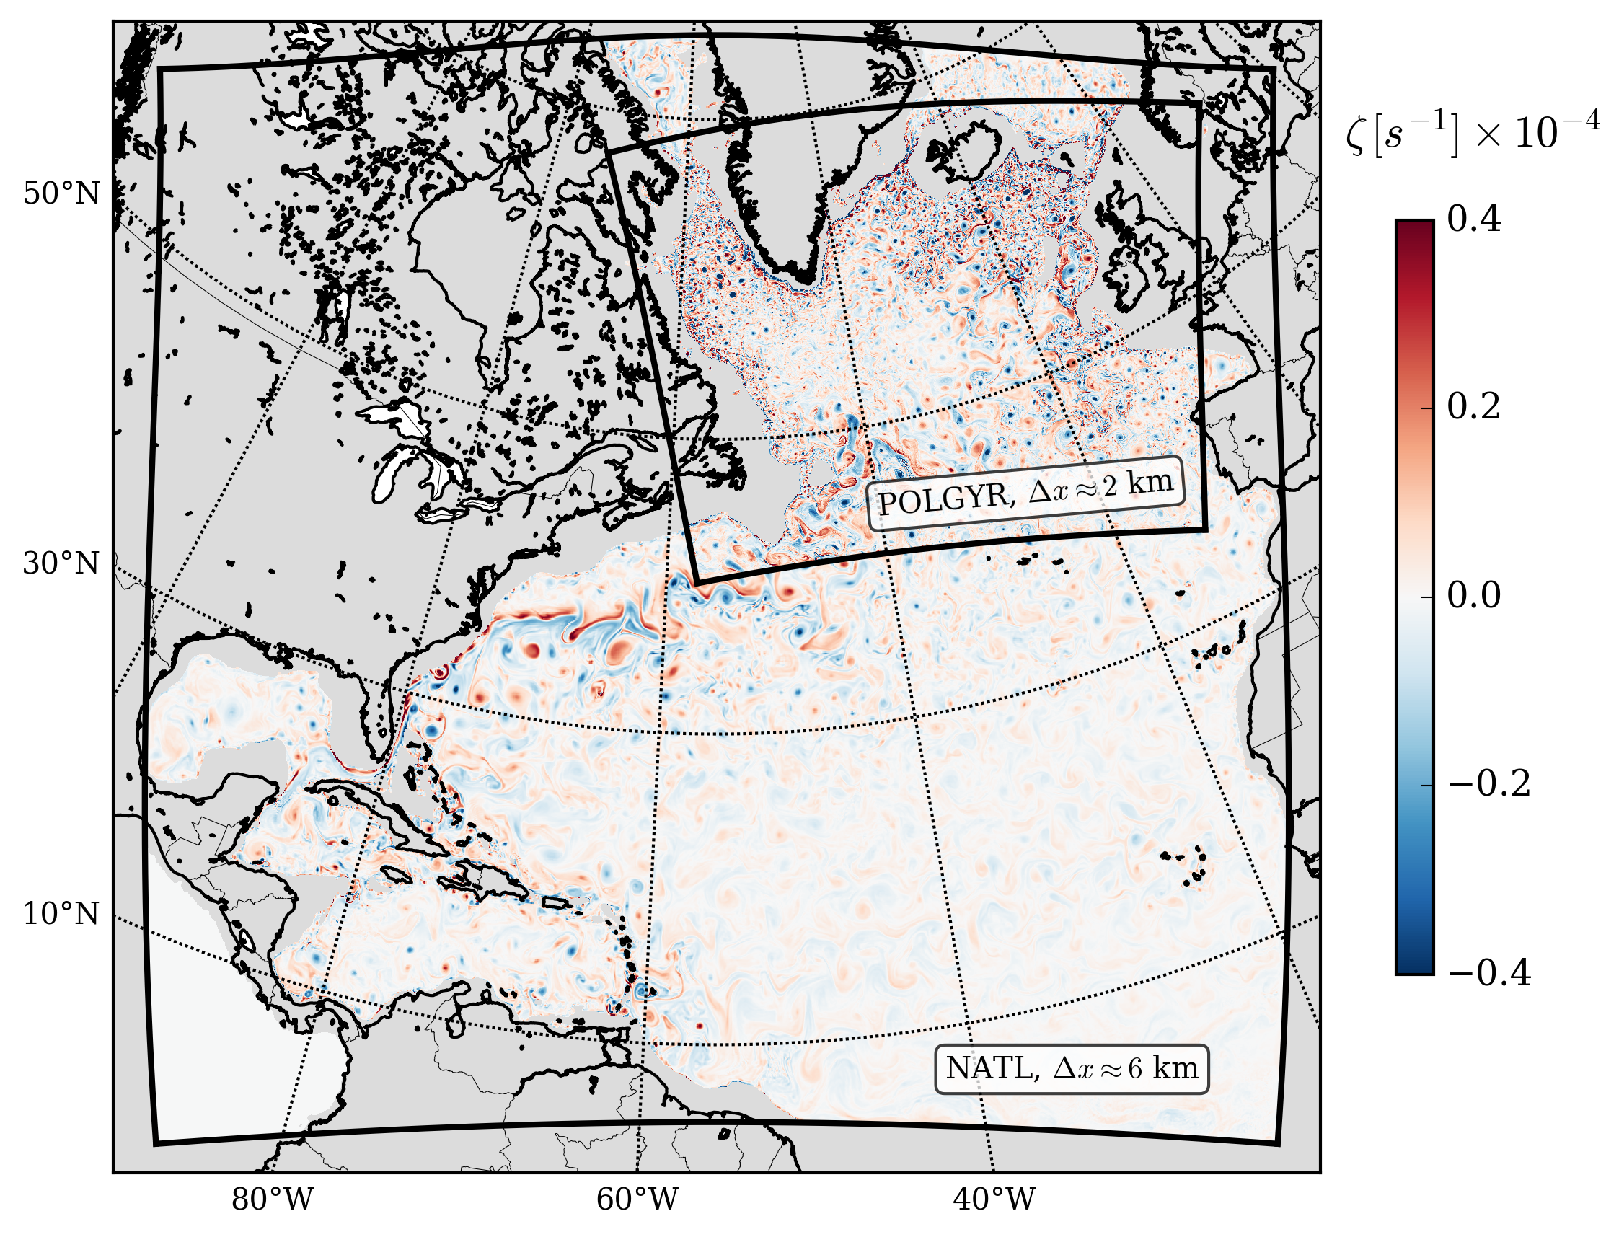
\includegraphics[width=10cm]{../fig_os/f01.pdf}
\caption{Snapshot of the relative vorticity at 500 m depth in the North Atlantic in the NATL simulation. The NATL grid ($\Delta x \approx 6$ km) covers most the North Atlantic, and the POLGYR grid (smaller rectangle, $\Delta x \approx 2$ km) covers the subpolar gyre.}
\label{f01}
\end{figure} 

The bathymetry for both domains is constructed from the SRTM30 PLUS dataset (available online at \url{http://topex.ucsd.edu/WWW_html/srtm30_plus.html}) based on the 1 min \cite{sandwell1997} global dataset and higher resolution data where available. A Gaussian smoothing kernel with a width 4 times the topographic grid spacing is used to avoid aliasing whenever the topographic data are available at higher resolution than the computational grid and to ensure the smoothness of the topography at the grid scale. Also, to avoid pressure gradient errors induced by terrain-following coordinates in shallow regions with steep bathymetric slopes \citep{beckmann1993}, we locally smooth the bottom topography $h$ to ensure that the steepness of the topography does not exceed a factor $r=0.2$, where the local $r$-factor is defined in the x and y directions by $r_x = \frac{h(i,j)-h(i-1,j)}{h(i,j)+h(i-1,j)}$ and $r_y = \frac{h(i,j)-h(i,j-1)}{h(i,j)+h(i,j-1)}$,  (i,j) representing the grid index.

Initial and lateral boundary data for the largest domain are taken from the Simple Ocean Data Assimilation (SODA, \citet{carton2008}). The NATL simulation is run from January 1st, 1999 to December 31st, 2009. It is spun up for 2 years, and the following 8 years are used to generate boundary conditions for the child grid. Our focus is the barotropic vorticity dynamics, characterized by time scales on the order of months, such that a year of spin up is sufficient for the kinetic energy to reach a state of quasi-equilibrium in POLGYR (not shown). The study is carried on the 7 remaining years between 2002 and 2009. The surface forcings are daily ERA-INTERIM data for the parent grid and 12-hourly ERA-INTERIM data for the child grid.

\begin{figure}[t]
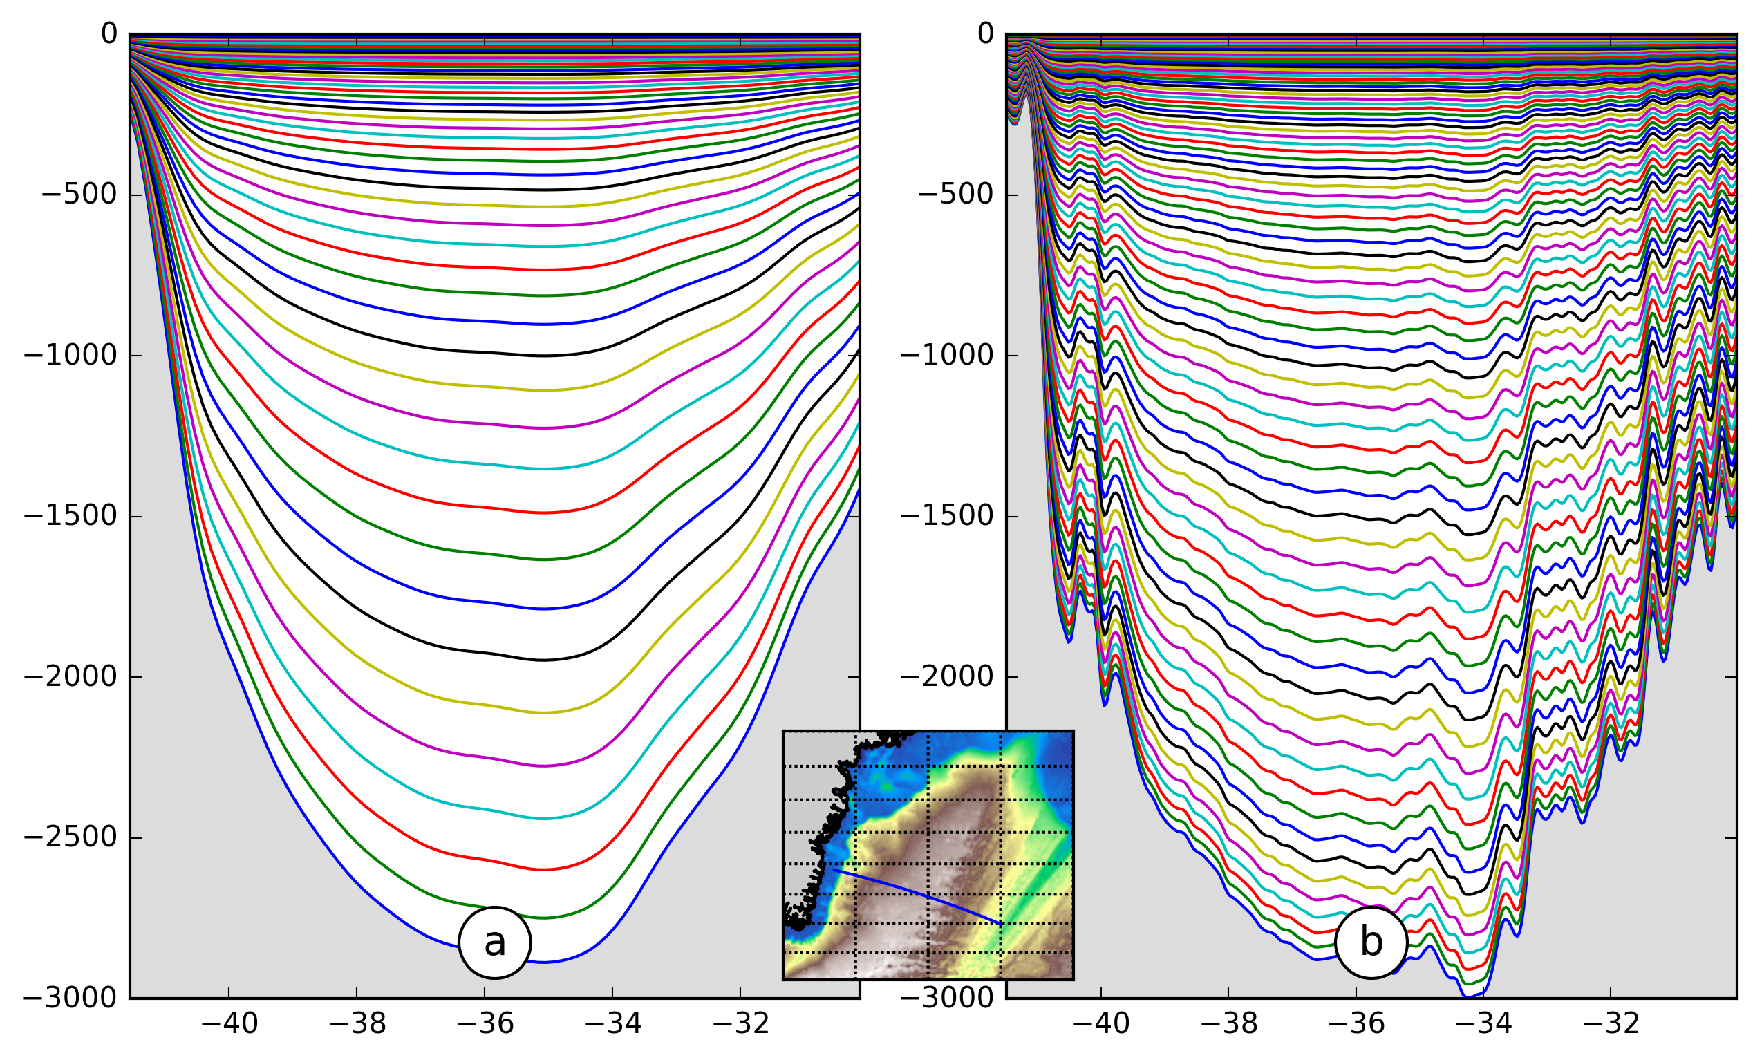
\includegraphics[width=8cm]{../fig_os/f02.pdf}
\caption{Depths of the model vertical $\sigma$-levels along a section in the Irminger Basin for (a) the 6-km simulation (NATL), and (b) the 2-km simulation (POLGYR).}
\label{f02}
\end{figure} 


The North Atlantic and subpolar gyre simulations have 50 and 80 vertical levels, respectively. Vertical levels are stretched at the surface and bottom \citep{lemarie2012} to have a better representation of the surface layer dynamics at the top and flow-topography interactions at the bottom. The depth of the transition between flat z levels and terrain-following $\sigma$ levels is $h_{cline} = 300$ m. The two parameters controlling the bottom and surface refinement of the grid are $\sigma _b=2$, $\sigma _s=7$ for the parent grid and $\sigma _b=3$, $\sigma _s=6$ for the child grid, corresponding to strongly stretched levels at the surface and bottom (Fig. \ref{f02}).

The vertical mixing of tracers and momentum is done by a k-$\epsilon$ model (GLS, \citet{umlauf2003}). The effect of bottom friction is parameterized through a logarithmic law of the wall with a roughness length $Z_{0} = 0.01$ m.% In addition the diffusion created by the numerical scheme is sufficient and do not require explicit horizontal viscosity.


\section{Mean Currents and variability}
\subsubsection{Mean circulation}
Before investigating what is driving the SPG dynamics, we first need to validate the mean circulation in our simulations. Mean velocities from the two simulations (NATL and POLGYR) at the surface and 1000-m depth are shown in figure \ref{f03}. We present at the bottom of figure \ref{f03} (e,f) the amplitudes of the currents from the NOAA drifter climatology \citep{laurindo2017} at the surface and from the ARGO-based ANDRO dataset at 1000-m depth \citep{ollitrault2013,lebedev2007}. The ANDRO data have been binned on a $0.25^{\circ}\times 0.25^{\circ}$ grid and cells with less than 10 data points have been removed. 

The North Atlantic Current (NAC) represents a boundary between the subtropical and the subpolar gyres. Oceanic models have difficulties in reproducing its dynamics and particularly its Northern extension known as the NorthWest Corner \citep{bryan2007,hecht2008,drews2015}, which is centered at 50$^{\circ}$ N, 48 $^{\circ}$ W \citep{lazier1994}. These difficulties lead to the apparition of the so called "cold-bias", which can reach up to 10 $^{\circ}$C \citep{griffies2009, drews2015}, and which plays a role in the Atlantic low frequency variability \citep{drews2017}. The NorthWest Corner is well reproduced in our simulations, and the temperature bias at this location is less than a degree.


After turning eastward, the NAC splits into three branches, which are strongly constrained by topography \citep{bower2008}. They cross the Mid Atlantic Ridge (MAR) through three deep fracture zones: the Charlie-Gibbs Fracture Zone (CGFZ, 52.5 $^{\circ}$ N), the Faraday fracture zone (50$^{\circ}$ N) and the Maxwell fracture zone (48$^{\circ}$ N) \citep{bower2002}. In both surface and 1000 m observations (Fig. \ref{f03}(e),(f)), the Northern branch of the NAC is more intense and corresponds to the main pathway across the MAR. The three branches are well represented in the simulations with, at the surface, an overestimation of the southern branch and an underestimation of the northern branch. At depth, ANDRO data depict an intense branch crossing the MAR at the CGFZ while the amplitude of the two Southern branches is smaller. This feature might be related to the Labrador Sea Water passing into the Eastern Basin through the CGFZ in this depth range, while in the Faraday and Maxwell Fracture zones the flow is more surface intensified. The circulation in POLGYR is closer to the observations with a better representation of the flow in the CGFZ at 1000 m. 

\begin{figure*}[t]
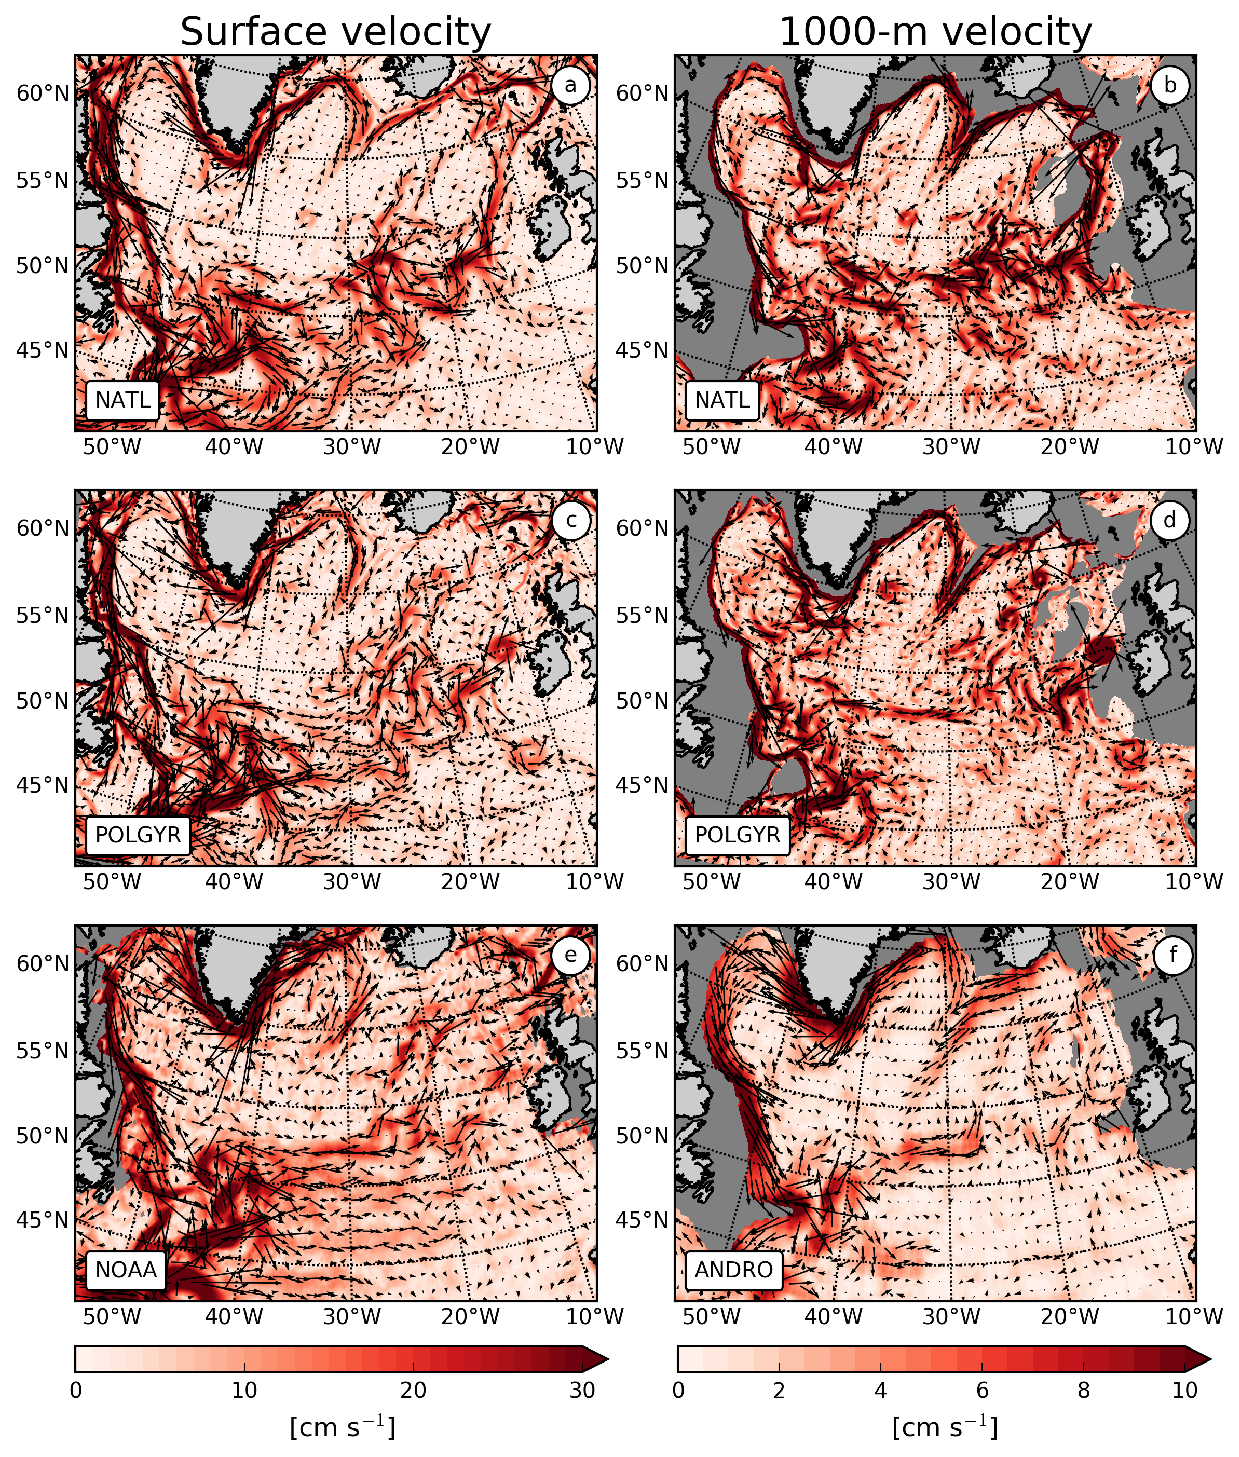
\includegraphics[width=15cm]{../fig_os/f03.pdf}
\caption{Mean velocity averaged over 2002-2008 at the surface (left) and 1000-m (right) in NATL (a,b), POLGYR (c,d) and observations, NOAA drifters and ANDRO (e,f).}
\label{f03}
\end{figure*}


After crossing the MAR, the three branches head North with the two Northern ones feeding the interior of the Iceland basin and the Rockall Trough (RT) \citep{daniault2016}. The water coming from the Maxwell fracture zone recirculates southward in the West European Basin \citep{paillet1997}. As most of the models \citep{treguier2005,deshayes2007}, NATL and POLGYR are consistent with observations for the circulation in the Eastern Basin  with a good positioning of the two main branches passing respectively in the Maury channel (deepest part of the Iceland Basin west of Hatton Bank) and the RT. 

A deep permanent anticyclonic eddy is found in Rockall Trough \citep{fischer2018,smilenova,lecorre2019}. This structure is detectable in the ANDRO dataset around 55$^{\circ}$ N, 12$^{\circ}$ W (Fig. \ref{f03}(f)). It is not present in NATL while it appears in POLGYR, albeit with too intense velocities. In NATL at depth, there is a strong southward flow in the western part of the RT due to the wrong representation of the Faroe Bank channel. As the topography is strongly smoothed, the channel is not properly represented and does not allow the dense water coming from the Nordic Seas to pass through it and feed the Iceland Scotland Overflow Water properly \citep{hansen2016,kanzow2014}. Thus, the water is recirculating in the western part of the RT, creating a spurious pattern (Fig. \ref{f03}(b)). The problem is solved by increasing the horizontal resolution and improving the representation of the topography, which corresponds to a wider opening of the channel and allows a more realistic circulation in the RT. 

Further north, part of the flow continues to the Nordic Seas \citep{rossby2012}, while the other part follows the Reykjanes Ridge (RR). A common bias in models east of RR is a too intense southward flow at the surface \citep{treguier2005}. This bias is present in NATL but disappears at higher resolution in POLGYR, which is closer to the circulation observed by the drifters. On the western side of the RR the signal of the strong northward Irminger current visible in observations is well resolved by the simulations (Fig. \ref{f03}). 

At 1000-m depth, Argo floats reveal a continuous current following the Eastern RR flank until reaching the CGFZ, with some of the flow crossing the ridge North of 57.3$^{\circ}$ N and some crossing at the Bight Fracture Zone (56-57$^{\circ}$ N). This is consistent with the results from \citet{petit2018}, who observed that water at this depth (their layer 3) was more likely to cross the ridge North of 56$^{\circ}$N. This southwestward flow is present in our simulations, with too intense velocity amplitudes in NATL, but realistic amplitudes at higher resolution in POLGYR. In both cases, we clearly see the flow crossing the ridge north of 56$^{\circ}$N. On the western side of RR, the velocity in the simulations is too strong compared to observations.
The mean subpolar gyre intensity in the model (Fig. \ref{f04}), computed as the cumulative transport from Iceland to 53.15$^{\circ}$ N along the crest of the RR, is equal to -25 Sv and compares well with the -21.9 $\pm$ 2.5 Sv monthly average in \citet{petit2018}.  

\begin{figure}[t]
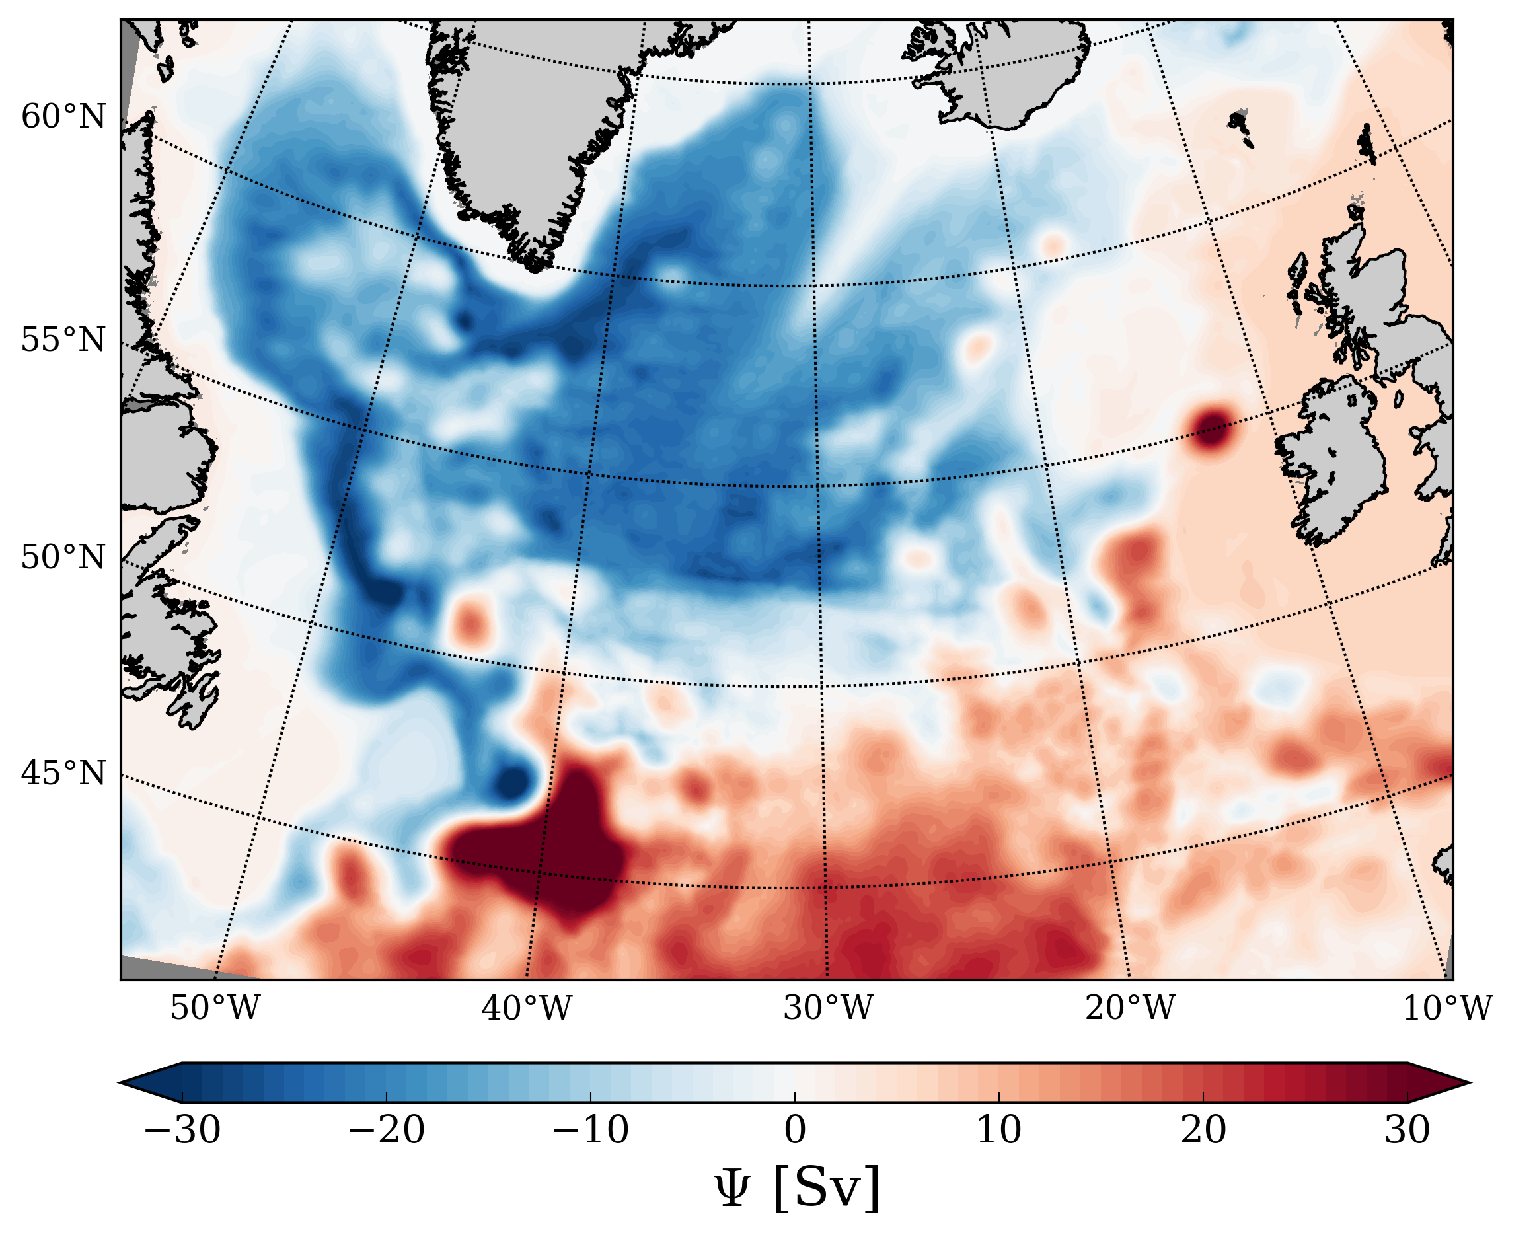
\includegraphics[width=8cm]{../fig_os/f04.pdf}
\caption{Time mean barotropic stream function over 2002-2008}
\label{f04}
\end{figure}

Numerous recirculations are present in the SPG, many of them occurring near the intense boundary currents along Greenland and around the Labrador sea \citep{reverdin2003, flatau2003,cuny2002}. The recirculation cells are present in the Labrador sea \citep{lavender2000,cuny2002} and extend to the Irminger basin \citep{Holliday2009}. \citet{kase2001,spall2003} suggested that both the topography and the wind are driving theses features which are stable in time \citep{palter2016}. More recently \citet{wang2017} showed the importance of the mean flow advection in these circulations. Some models are unable to reproduce correctly the recirculation cells, especially the one in the centre of the Labrador Sea \citep{treguier2005}. In our case, this recirculation is well represented (Figure \ref{f03}(a),(b),(c),(d)). The counter current flows offshore the Labrador continental slope, with a northward extension at 60$^{\circ}$ N, which matches observations from \citet{lavender2005}.  At the tip of Greenland, this counter current separates in two to form a branch flowing inside the Irminger Basin while the other branch is redirected southward. This second branch is relatively intense in our simulation but is also present in ANDRO data (\cite{fischer2018}, their Figures 3 and 5a).  

\subsection{The mesoscale activity}

The mesoscale activity plays a big role in redistributing water masses properties in the SPG \citep{brandt2004,dejong2016,zhao2018b}. The presence of mesoscale eddies can be inferred by their signatures on the Eddy Kinetic Energy (EKE). From the surface EKE signal extracted from NOAA drifters on a $0.25^{\circ}\times 0.25^{\circ}$ grid (Fig. \ref{f05}(e)), we retrieve the main hot spots described by \citet{flatau2003} in the SPG: the Labrador Sea, the Irminger and Iceland basins. Those signals are mainly due to generation of mesoscale eddies through baroclinic and barotropic instabilities of the boundary currents.

\begin{figure*}[t]
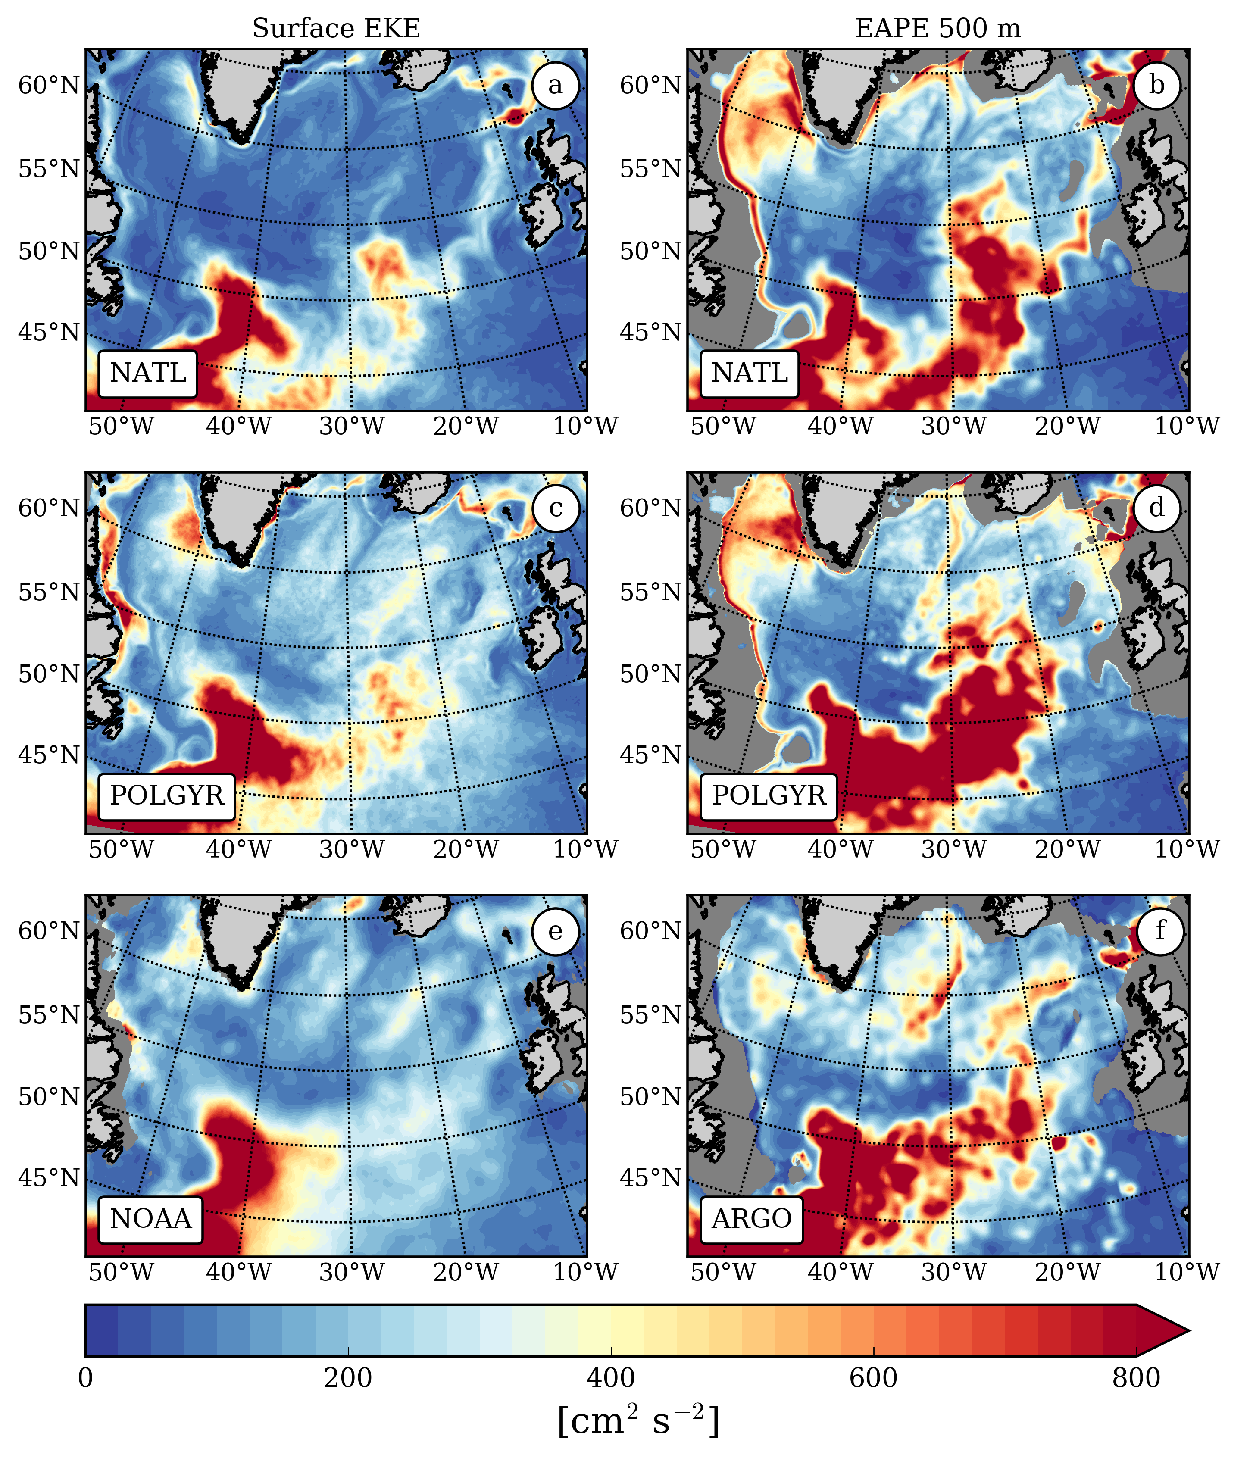
\includegraphics[width=15cm]{../fig_os/f05.pdf}
\caption{Mean Surface Eddy Kinetic Energy (left) and Mean Eddy Available Potential Energy between 2002 and 2008 (right) in NATL (a,b), POLGYR (c,d). There are compared with result from the NOAA database (e) and the EAPE Atlas from Roullet$\&$al (f)}
\label{f05}
\end{figure*}

EKE amplitudes in the NATL simulation are weaker than in observations, but the eddy activity is enhanced when the resolution is increased. The POLGYR simulation displays similar EKE patterns than observational data in every basins (Labrador, Irminger and Iceland) with close amplitudes over most of the SPG. The EKE patterns corresponding to the generation of Irminger Rings have higher magnitudes in POLGYR than in the NOAA drifters data.

A way to quantify the mesoscale activity at depth is to look at the vertical isopycnal displacements. When referenced to a mean, it represents the Eddy Available Potential Energy (EAPE) or the amount of energy stored in the potential energy reservoir due to mesoscale activity \citep{lorenz1955}. This quantity is a proxy of the baroclinic activity in the interior of the ocean and is computed following \citet{roullet2014} formulation:

\begin{equation}
    EAPE = - \frac{g}{2\rho _0} \langle z' \rho ' \rangle
\end{equation}

Where $z'$ is the vertical isopycnal displacement, $\rho '$ the density anomaly associated with this displacement and $\langle \bullet\rangle$ is the time average. We compare EAPE from the simulations with the atlas of \citet{roullet2014} constructed from Argo data (Fig. \ref{f05}(f)). The atlas presented here is an update of the original product by replacing virtual density by potential density and including more recent data up to July 2015. A basin-scale view of EAPE at. In NATL (at 6 km resolution) most of the baroclinic activity already seems well resolved. However, observations highlight an EAPE maximum on the western flank of the RR that is missing in NATL, but appears only in POLGYR (at 2 km resolution). On the contrary, strong patches of EAPE are visible along the boundary currents of the western half of the SPG in NATL, but are not visible in observations. Interestingly these patterns weaken in POLGYR, potentially pointing to a change in the vertical structure of the currents at higher resolution. Another factor to take into consideration is the lack of Argo measurements close to the boundaries, which might cause an underestimation of EAPE at these locations.

\section{Vorticity balance of the subpolar gyre at high resolution}
\subsection{An overall view of the subpolar gyre vorticity balance}

The barotropic vorticity equation is obtained by integrating the momentum equations in the vertical and cross-differentiating them \citep{gula2015}:

\begin{equation}
\underbrace{\frac{\partial \Omega}{\partial t}}_{rate} = -\underbrace{\mathbf{\nabla}.(f \mathbf{\overline{u}})}_{planet.\;vort.\;adv}+\underbrace{\frac{J(P_b,h)}{\rho _0}}_{BPT} +\underbrace{\mathbf{k}.\mathbf{\nabla} \times \frac{\mathbf{\tau} _{wind}}{\rho_{0}}}_{wind\;curl} -\underbrace{\mathbf{k} \cdot \mathbf{\nabla} \times \frac{\mathbf{\tau} _{bot}}{\rho_{0}}}_{BDC} +\underbrace{D_{\Sigma}}_{horiz.\;diffusion}+\underbrace{A_{\Sigma}}_{NLA}
\end{equation}


where the vorticity $\Omega$ is the curl of the vertically integrated components of the velocity between the bottom and the surface: $\Omega = \mathbf{k} \cdot \mathbf{\nabla} \times \overline{\mathbf{u}}$, with $\mathbf{u} = (u,v)$ the velocities in the $(x,y)$ direction. The overbar defines a vertically integrated quantity:

\begin{equation}
\overline{u}=\int^{\eta}_{-h} u \; dz
\end{equation}
with $\eta(x,y,t)$ the free surface height and $h(x,y)$ the topography. It is possible to decompose the planetary vorticity advection $-\nabla.(f\overline{u})=-\beta V-f \frac{\partial \eta}{\partial t}\approx - \beta V$, with $V$ the vertically integrated meridional component of velocity, if we consider a mean over a long enough time period such that $\frac{\partial \eta}{\partial t} \approx 0$.

The non linear term can be written as:

\begin{equation}
A_{\Sigma}= -\frac{\partial ^2 (\overline{vv}-\overline{uu})}{\partial x \partial y}-\frac{\partial ^2 \overline{uv}}{\partial x \partial x} +\frac{\partial ^2 \overline{uv}}{\partial y \partial y}
\end{equation}

The expression for $A_{\Sigma}$ is similar to the one shown in \citet{schoonover2016} (their equation (2)) but in our case, the integration between -h and $\eta$ allows their last term to cancel out with a residue from the inversion of the time derivative and the vertical integral in the rate term. The bottom pressure torque J(P$_b$,h) is the Jacobian of the bottom pressure and the depth of the topography. It encompasses the effects of the varying topography on the flow, and is known to play a key role in the barotropic vorticity balance of the SPG. In an idealized case of a geostrophic current flowing along a topography in free-slip condition, the BPT can be written $\frac{J(P_b,h)}{\rho _0}=f u_b \cdot \nabla h$ where $\rho_0$ is the mean reference density and the subscript $b$ denotes a field at the bottom. Given the kinematic condition at the bottom: $-u_b \cdot \nabla h =w_b$, the BPT can be written $\frac{J(P_b,h)}{\rho _0}=-fw_b$, which highlights the relation between the BPT and vortex stretching when the flow crosses an isobath.

The barotropic vorticity terms have already been computed for the North Atlantic using different models (Ocean Circulation and Climate Advanced Modelling- OCCAM; Estimating the Circulation and Climate of the Ocean- ECCO \cite{wunsch2013}; University of Victoria Earth System Climate Model- UVic ESCM \cite{weaver2001}; Parallel Ocean Program-POP \cite{smith2010}) at different resolutions ($1.8^{\circ}\times3.6^{\circ}$, $1^{\circ}$, $0.25^{\circ}$, $0.2^{\circ}\times 0.4^{\circ}$, $0.1^{\circ}$) in \citet{hughes2001}, \citet{spence2012}, \citet{sonnewald2019}, and \citet{yeager2015}. Their major result is that the barotropic vorticity balance in the subtropical and subpolar gyres is at first order a balance between $\beta$V, $\nabla \times \frac{\tau _{wind}}{\rho_{0}}$, and $\frac{J(P_b,h)}{\rho _0}$. 

In the subtropical gyre, the barotropic vorticity balance is close to a Sverdrup balance away from the boundaries ($\beta V \approx \nabla \times \frac{\tau _{wind}}{\rho_{0}}$), while the closure of the northward branch of the gyre at the western boundary is done primarily through BPT ($\beta V \approx \frac{J(P_b,h)}{\rho _0}$)  \citep{schoonover2016}.

The barotropic vorticity balance in the SPG is slightly more complex due to the strong impact of the topography. Along the northern and western boundaries of the SPG, the first order balance is between meridional advection and BPT ($\beta V \approx \frac{J(P_b,h)}{\rho _0}$) (\textit{e.g.} \citet{hughes2001}, their Figure 4; \citet{yeager2015}, their Figure 1), with a significant impact of the wind only in the northern part of the gyre along the Greenland coast. When the resolution of the model is increased from $1^{\circ}$ to $0.1^{\circ}$ in \citet{yeager2015}, the main balances stay qualitatively similar, showing a modest effect of the eddies. Using a shallow water model with higher resolution ($1/20^{\circ}$), \cite{wang2017} illustrates the importance of the NL term in the dynamics of specific regions such as the Gulf Stream and the Labrador recirculation in the SPG. The viscous torque decreases in the boundary currents due to the lower viscosity of their model.

\subsection{Spatial scales of the vorticity balance}

In our simulations, the BPT balances the nonlinear term at leading order everywhere in the domain  (Fig. \ref{f06}). This is qualitatively different from the vorticity balances shown in \citet{yeager2015}, but it is similar to the results of \citet{gula2015} in the Gulf Stream region with the same ocean model and a similar horizontal resolution. This highlights the fact that locally the flow is able to follow isobaths due to an equilibrium between the NL term (making the flow cross isobaths) and the bottom pressure anomaly.

Both terms exhibit small scales related to topographic features, but with a high degree of cancellation between each other. The sum of the BPT and NL terms (Fig. \ref{f06} (c) is often an order of magnitude smaller than the amplitude of the terms considered individually and exhibits patterns and amplitudes matching the advection of planetary vorticity. This cancellation is also clear in \cite{wang2017}, their Figure 3, where the transport driven by mean flow advection balances the one driven by the BPT, both having amplitudes larger than the wind stress curl-driven transport.

\begin{figure*}[t]
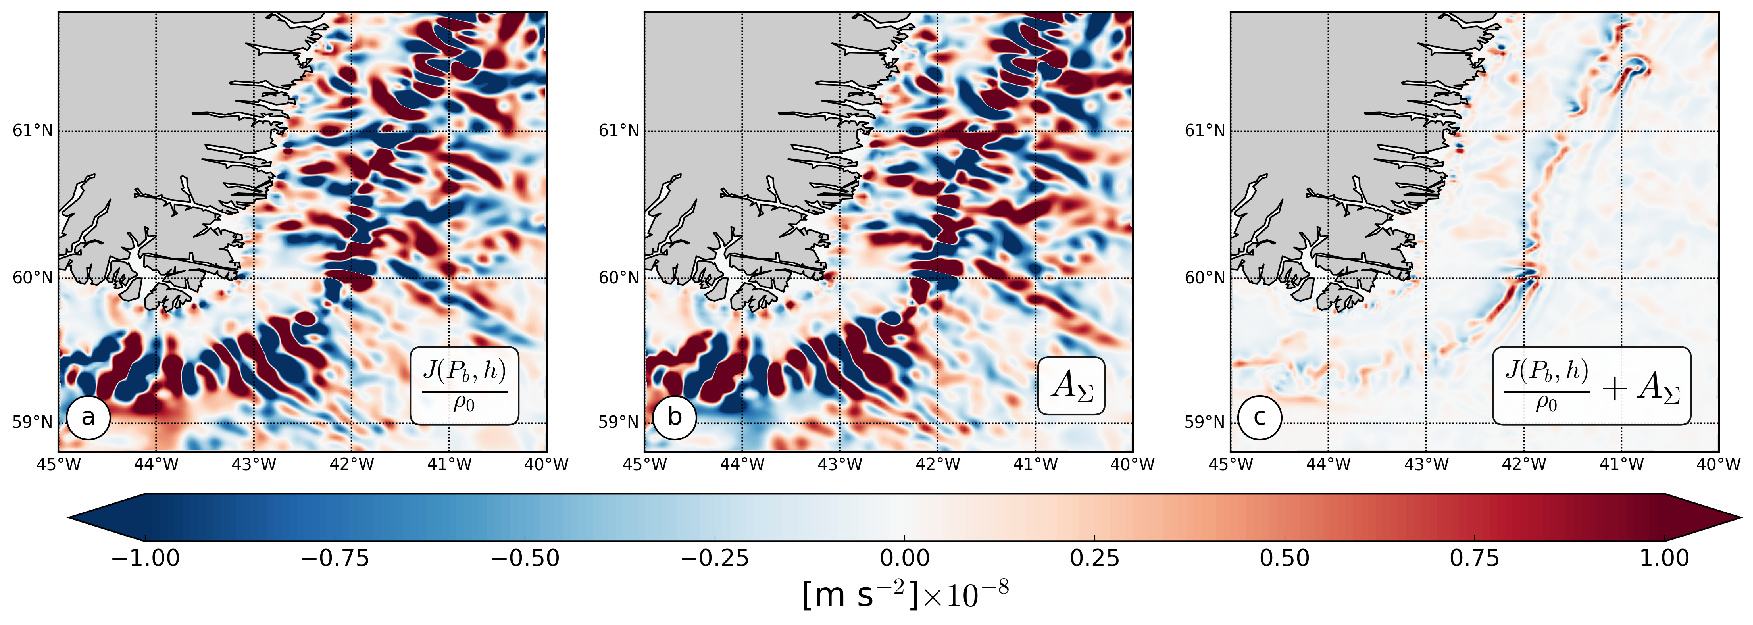
\includegraphics[width=15cm]{../fig_os/f06.pdf}
\caption{Time mean (a) bottom pressure torque, (b) non-linear terms, and (c) sum of the two for Eastern Greenland in the 2-km North Atlantic subpolar gyre simulation.}
\label{f06}
\end{figure*} 

To facilitate the interpretation of maps of NL and BPT terms, the impact of small topographic scales has to be reduced by smoothing with a large enough length scale. 
NL terms in particular are expected to be smoothed out on scales larger than 1-2$^{\circ}$ \citep{hughes2001}. Figure \ref{f07} shows all terms smoothed with a Gaussian kernel of 1$^{\circ}$ radius. Even with such smoothing, the BPT and NL terms are still significantly larger than the corresponding results from the $0.1^{\circ}$ simulation of \citet{yeager2015}. However, their sum $\frac{J(P_b,h)}{\rho _0}+A_{\Sigma}$ (Fig. \ref{f07} (f)) is of the same order of magnitude than the $\beta$V (Fig. \ref{f07} (a) ) and the Bottom Drag Curl (BDC, Fig. \ref{f07} (e)). 

\begin{figure*}[t]
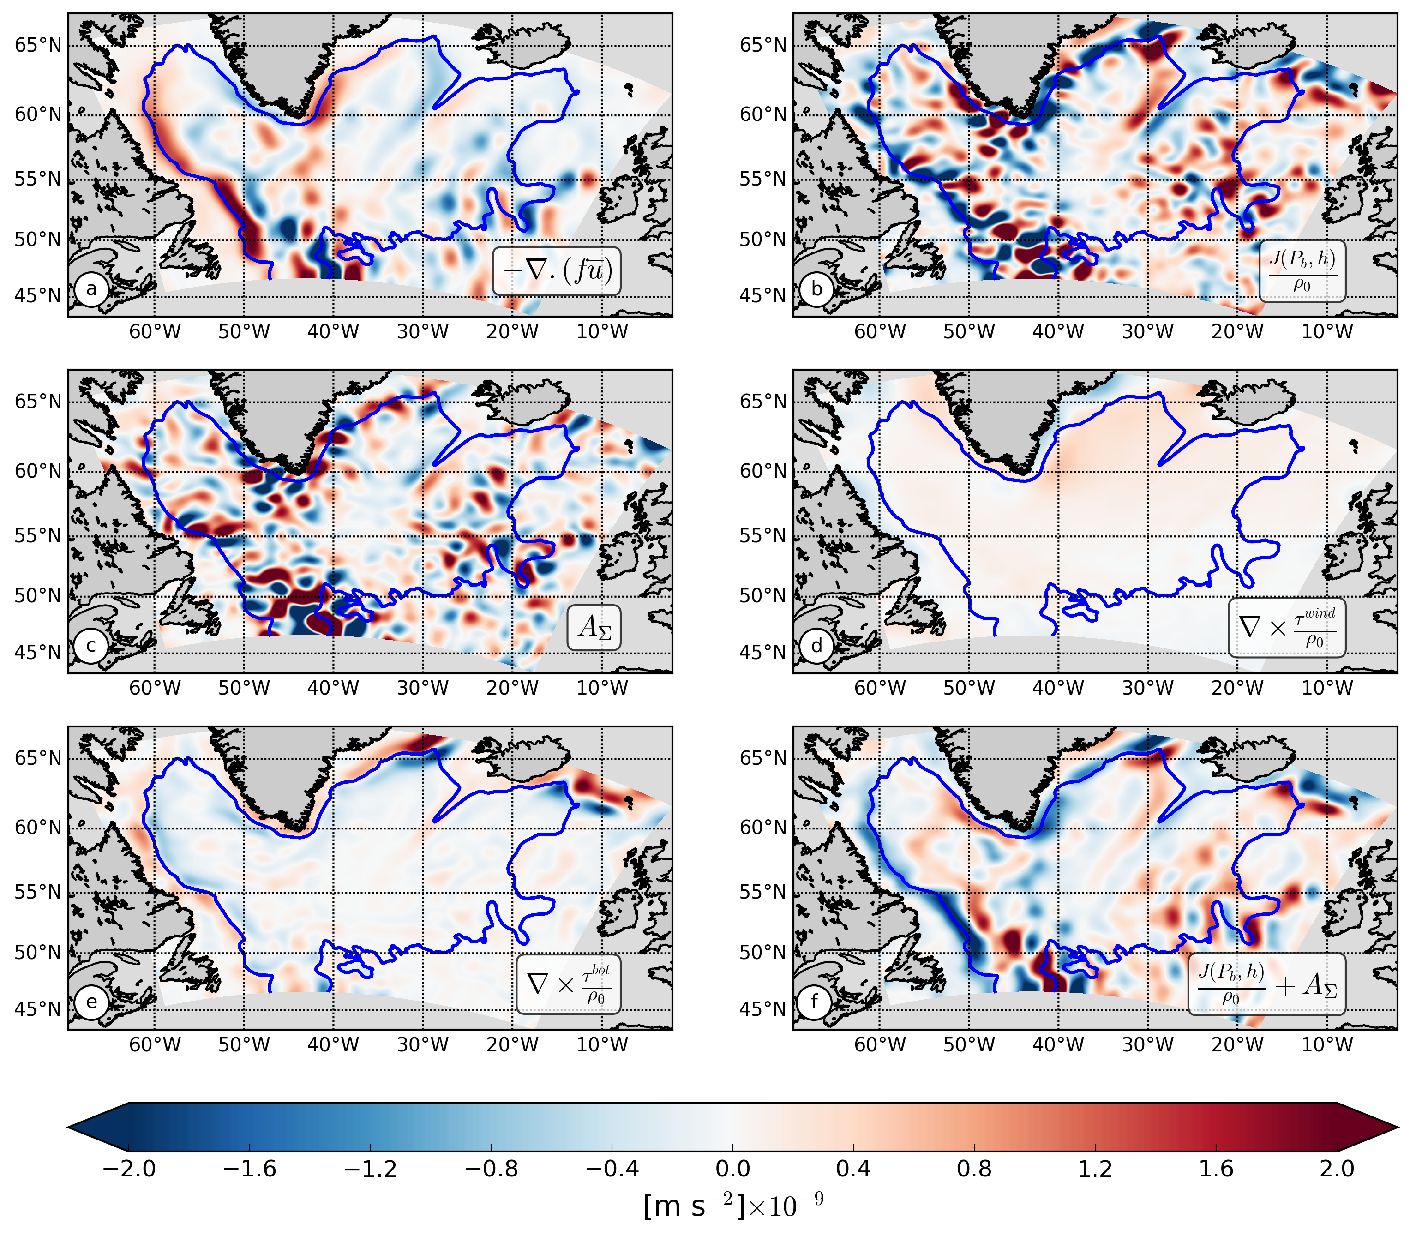
\includegraphics[width=15cm]{../fig_os/f07.pdf}
\caption{ Time mean of the planetary vorticity (a), bottom pressure torque (b), non linear terms (c), wind stress curl (d), and bottom drag curl (e). As bottom pressure torque and non-linear terms are canceling each other their sum is plotted in (f). The fields have been smoothed using a kernel of 1$^{\circ}$ radius. The blue contour represents the limit of our shelf area and is the -3 Sv barotropic streamline}
\label{f07}
\end{figure*} 

The curl of the wind stress in POLGYR has the same pattern and amplitude as in \citet{yeager2015}. It is mostly positive with the strongest signal on the Eastern coast of Greenland. The amplitude of the $\beta$V term is slightly stronger in our model than in coarser resolution simulations. In the simulations of \citet{hughes2001} and \citet{yeager2015}, the patterns of the $\beta$V term seems to indicate much wider currents. Here, the patterns correspond to thinner and more intense currents, closely following the continental slopes, in agreement with the observations.

In our simulations, the amplitude of the viscous torque, due to the horizontal viscosity of the model ($D_{\Sigma}$), is very small, while the amplitude of the BDC is comparable to the $\beta V$. This is opposite to the results of the $0.1^{\circ}$ POP simulation of \citet{yeager2015}. In fact, their viscous term is qualitatively similar in pattern to the bottom drag curl in our simulation. The boundary conditions near the topography are quite different in the two models due to the different vertical coordinates. The z-levels coordinates have vertical walls between each level, with parameterized lateral viscosity, which explains the pattern in \citet{yeager2015}. The $\sigma$-levels coordinates have no lateral boundary conditions and friction on the topographic slopes is only parameterized as a bottom drag. The amplitude of the BDC is however stronger in our simulation than the viscous term in \citet{yeager2015} and seems to play a important role in balancing the BPT and $\beta V$ terms over the shelf and on the upper part of the continental slope along the northern and western boundaries of the gyre.

\subsection{Link between barotropic vorticity balance and bottom velocities}

As explained previously, the bottom pressure torque J(P$_b$,h) can be identified with a bottom vortex stretching term: $\frac{J(P_b,h)}{\rho _0}=f u_{gb}.\nabla h = -f w_{gb}$, where $u_{gb}$ is the horizontal geostrophic bottom flow. 

The computation of the BPT in \citet{spence2012} is performed by directly estimating the term  $-f w_{b}$, where $w_{b}$ is the vertical velocity at the bottom. However this estimation does not take into account the presence of an ageostrophic component of the velocity at the bottom, in particular the Ekman component of the velocity due to the bottom drag. The same computation in our model leads to the results of Fig. \ref{f08}(b), which are very different from the actual bottom pressure torque (Fig. \ref{f08} (a)). It gives results quite similar to \citet{spence2012} with positive signals - implying downwelling of bottom currents - over most of the boundaries of the gyre. But this downwelling is a result of the Ekman currents oriented to the left of the main bottom geostrophic currents, which are flowing with the shallower topography on their right around the gyre.


\begin{figure*}[t]
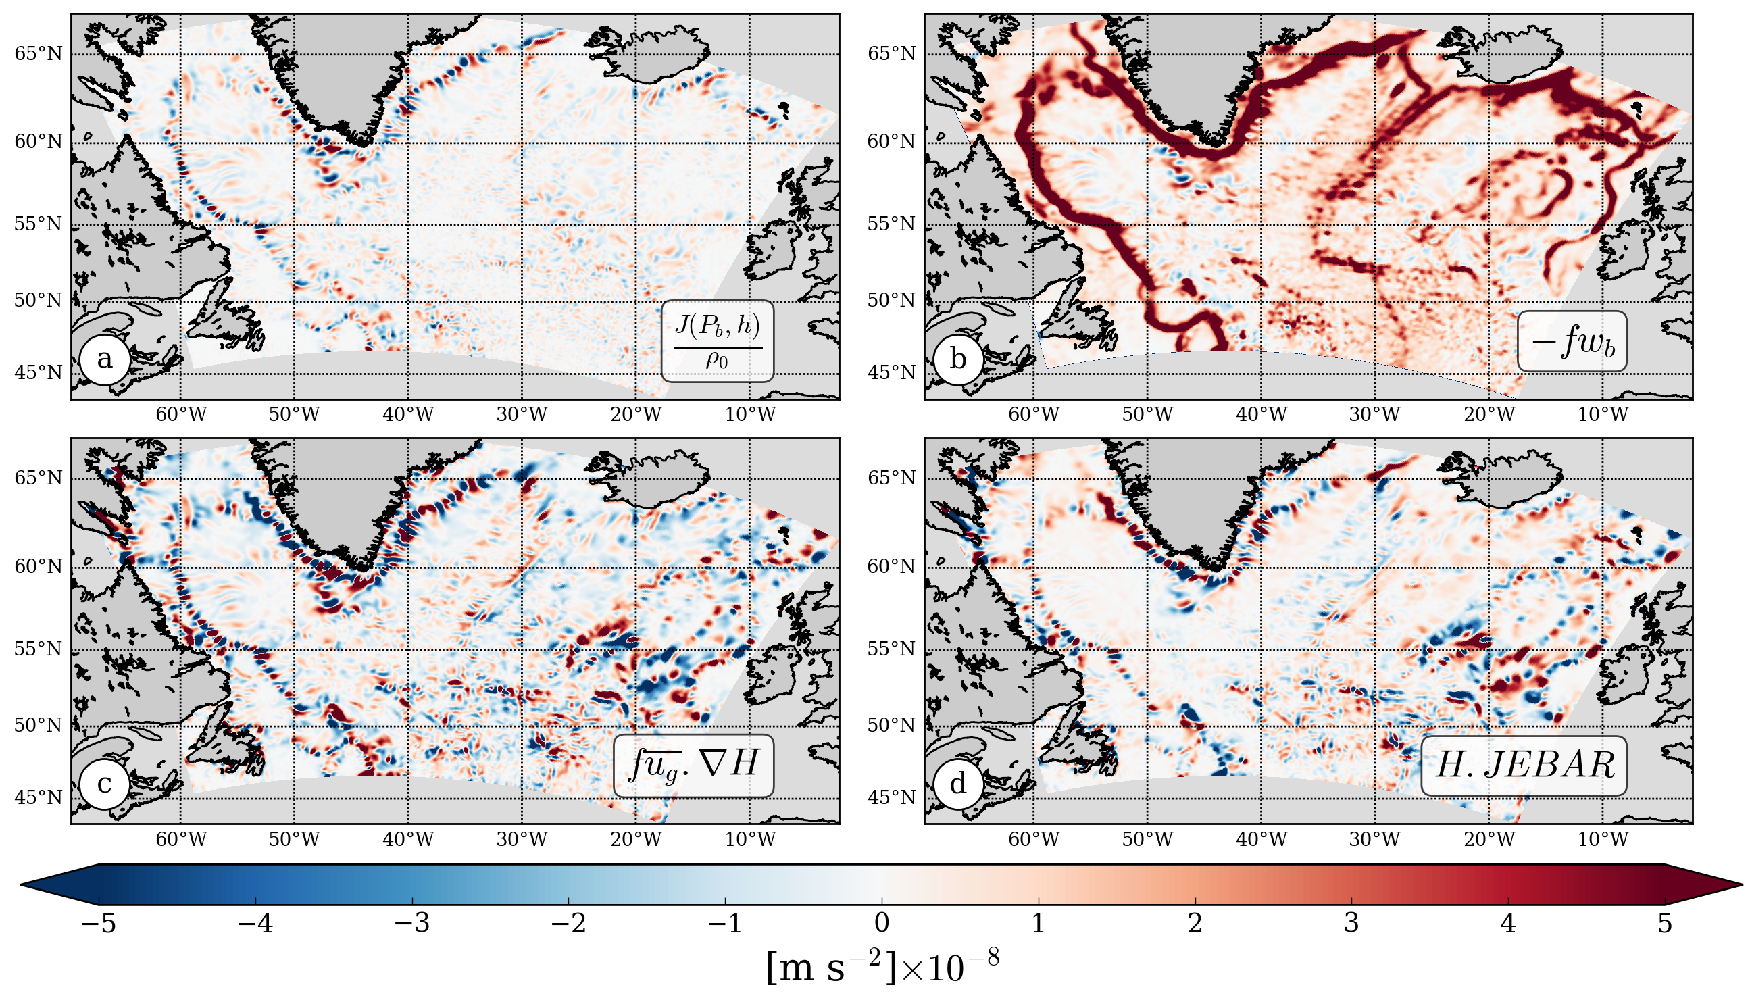
\includegraphics[width=15cm]{../fig_os/f08.pdf}
\caption{(a) Bottom Pressure Torque, (b) $-fw_b$, (c)$\frac{f}{h} \overline{u_g} \cdot \nabla H$, and (d) $H \cdot JEBAR$ for the 2-km North Atlantic subpolar gyre simulation smoothed with a 25 km Gaussian Kernel .}
\label{f08}
\end{figure*} 

Following \citet{mertz1992} and \citet{yeager2015}, the BPT can be further decomposed into:
\begin{equation}
\frac{J(P_b,h)}{\rho _0}=f u_{gb}.\nabla h = \frac{f}{h} \overline{u_g}.\nabla h +  h(JEBAR)
\end{equation}
which illustrates that the bottom geostrophic currents that appears in the expression of BPT are the sum of a vertically averaged part and a baroclinic part directly related to the JEBAR term. The term $ \frac{f}{h} \overline{u_g} \cdot \nabla h$ highlights regions where the depth-averaged flow is crossing isobaths, and the $h(JEBAR)$ term where the baroclinic effects are playing a role to decouple the bottom flow from the barotropic flow through the geostrophic shear. In Fig. \ref{f08} (c) the geostrophic velocity has been computed from the thermal wind balance referenced at the surface.

Along the continental slopes, on the western and northern part of the gyre, the flow is close to barotropic and the $ \frac{f}{h} \overline{u_g} \cdot \nabla H$ term has similar patterns and amplitudes than the BPT. This contrasts with results from \citet{yeager2015}, who found that the $h(JEBAR)$ term was almost an order of magnitude larger than the BPT in these regions. However over the southern and eastern part of the gyre, it is clear that the structure of the flow is much more baroclinic and the $ \frac{f}{h} \overline{u} \cdot \nabla h$ and  $h(JEBAR)$ terms are both an order of magnitude larger than the BPT.

\section{Integrated vorticity balance for the shelf, slope and interior of the gyre}
\subsection{Gyre integrated barotropic vorticity balances}

The maps of the barotropic vorticity terms, with various degrees of smoothing, can help identify the locally dominant terms, but do not enable us to identify the important balances at the gyre scale. Spatial integrations are performed inside different gyre contours (Fig. \ref{f09}) to better understand the main contributions to the circulation of the subpolar gyre. 

\begin{figure*}[t]
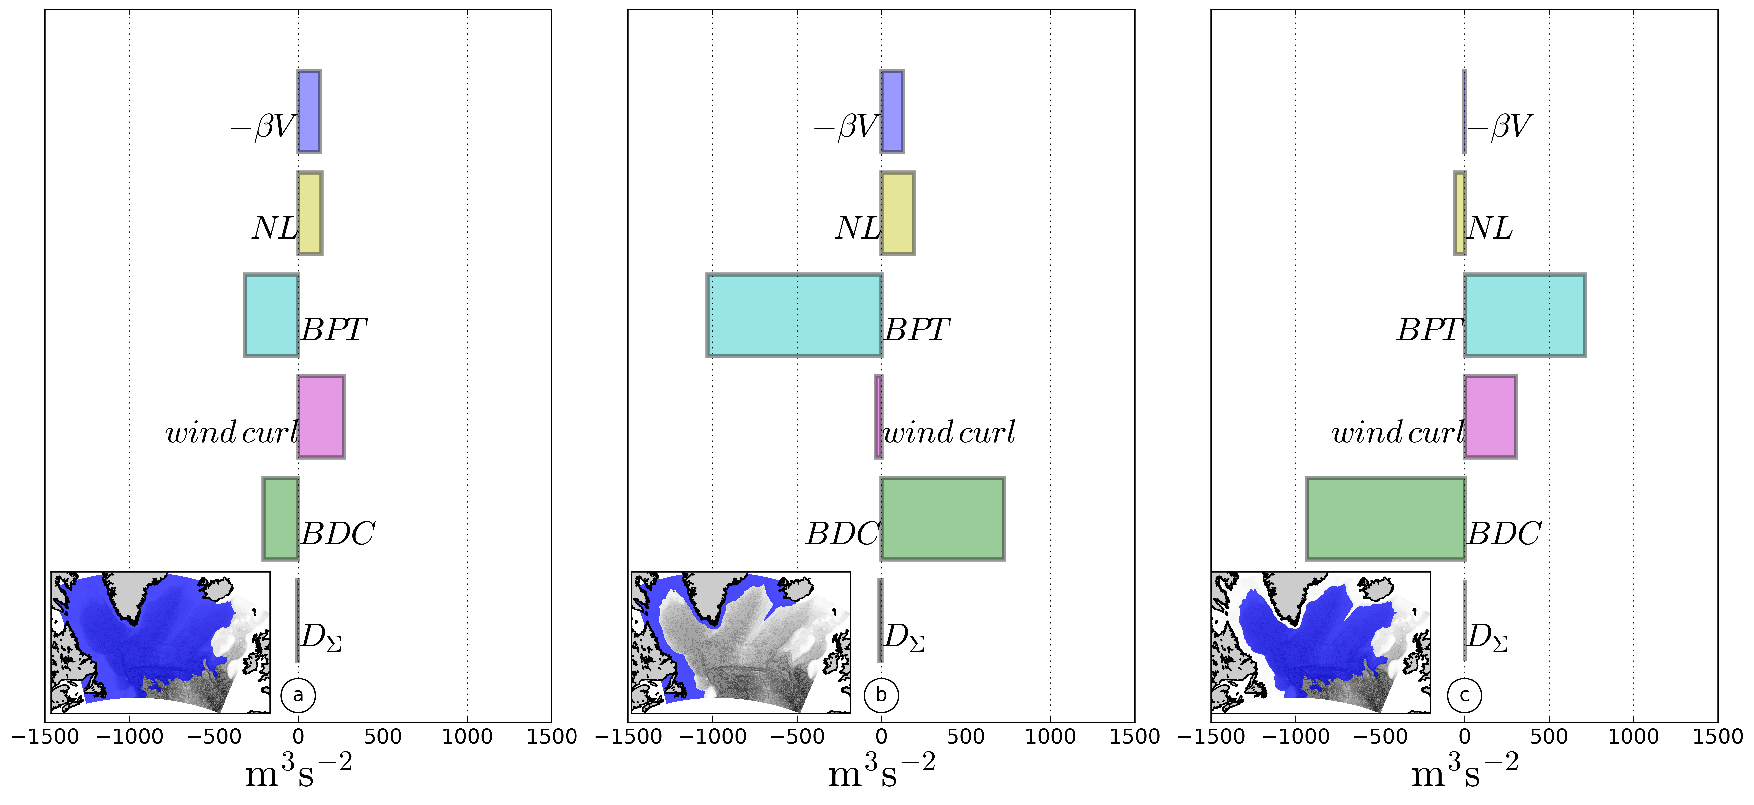
\includegraphics[width=14cm]{../fig_os/f09.pdf}
\caption{Integration of the barotropic vorticity terms over the SPG including or excluding the shelf area (respectively (a) and (c)). The Subpolar gyre area without the shelf corresponds to the -3 Sv contour. The shelf balance is plotted in (b).}
\label{f09}
\end{figure*} 

We distinguish the shelf area from the gyre using a contour of barotropic streamfunction of -3 Sv. This contour is chosen because it corresponds to the largest possible closed contour of the barotropic streamfunction. We can check that the term $-\nabla.(f\overline{u}) \approx -\beta$V integrates to zero within such a contour (Fig. \ref{f09} (c). The shelf thus defined corresponds to an area with a mean depth of 290 meter and is extending from the South of Iceland to Flemish cap (blue area in Fig. \ref{f09} (b)).

When integrated inside the -3 Sv contour (which means excluding the shelf area, Fig. \ref{f09} (c)), the main sources for the cyclonic circulation of the gyre are the wind and the BPT. They are balanced by the BDC. The wind input does not contribute much locally (Fig. \ref{f07}), but becomes significant when integrated spatially over the whole gyre. The BPT is the major source of positive vorticity and helps the flow move cyclonically around the gyre. The BDC and NL terms act as sinks of vorticity, but the NL term is much smaller than the BDC. The BDC is very intense where the current flows close to a steep topography, as in the case of the Labrador Current (LC) and the West Greenland Current. 

When integrated over the whole gyre (Fig. \ref{f09} (a)), the balance is slightly different. The wind is still a major contributor for the cyclonic circulation and the BDC still represents the major sink of vorticity. However, the NL term replaces the BPT as a source of cyclonic vorticity for the gyre. In this interpretation, both the wind and the NL term forces the gyre cyclonically, while the BDC and BPT balance this input. 


The difference between the two balances is highlighted by looking at the balance in the region in-between the two contours, which covers the upper slope and the shelf. It corresponds to a balance between BPT, NL and bottom drag. The NL term is only significant around Greenland shelf and is related to eddies interactions between shelf and open ocean. Otherwise, the vorticity is negative on the shelf thus explaining the positive sign of the bottom drag. The main source of anticyclonic vorticity is related to the BPT. This balance is close to the one described in \citet{csanady1978,csanady1997} and evokes a buoyancy driven flow in this area \citep{chapman1986,chapman1989}.

%Indeed, with a switch to ($n$,$s$) coordinates system with $n$ the right handed coordinates (here oriented toward shallower water) and $s$ the distance along flow, the BPT can be written $\frac{J(P_b,h)}{\rho _0}=-\frac{\partial P_b}{\partial s }\frac{\partial h}{\partial n}$. A negative value of BPT then means $\frac{\partial P_b}{\partial s }<0$ corresponding to a buoyancy driven current. 


\subsection{Barotropic vorticity balance in the interior of the gyre}

It is clear from the patterns of the different terms of the barotropic vorticity balance that the local balances over the boundary currents are very different than what is happening in the interior of the gyre. The classical picture of a gyre interior (far from the boundaries) in a quasi-Sverdrup balance that applies in the subtropical gyre,  does not seem to apply anywhere in the SPG. 

To better understand what drives the interior part of the subpolar gyre, we further divide the domain into an interior and a boundary part, as represented in Fig. \ref{f10}. The two domains are defined using the -3 Sv line as previously, and the 3000 m isobath. What is between the -3 Sv line and the 3000 m isobath is considered as the slope region and the rest is considered as the interior area. The choice of the 3000 m isobath is somehow subjective but the results are not sensitive to the choice of a specific isobath. 

\begin{figure*}[t]
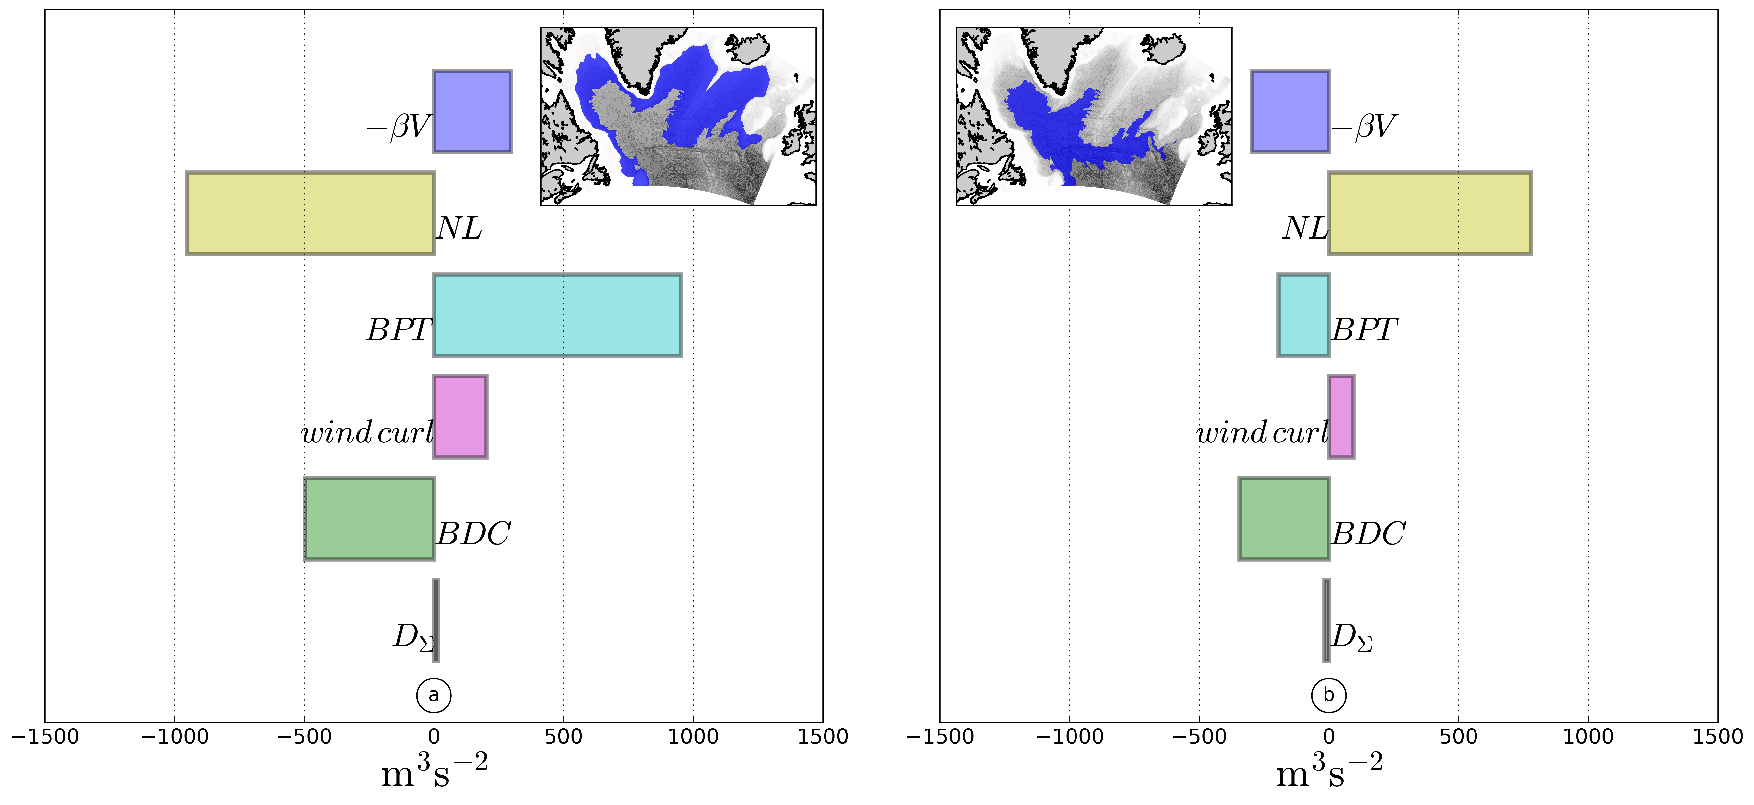
\includegraphics[width=14cm]{../fig_os/f10.pdf}
\caption{Integration of the barotropic vorticity terms in the slope area (a, defined between the barotropic streamfunction contour -3 Sv and the 3000-m isobath) and interior (b).}
\label{f10}
\end{figure*} 

In the slope region, the main source of cyclonic vorticity is the BPT. The curl of the wind and the $\beta$V are also positive. The strongly negative NL term indicates advection of cyclonic vorticity outside of this domain toward the shelf or the gyre interior.

In the interior, the NL term represents the major contribution to the cyclonic circulation. It is balanced by the BDC, the BPT and the $\beta$V terms. Contributions from the BDC are of similar magnitude in the interior and the slope area. The wind input of vorticity is smaller than in the slope region, as the major wind source of vorticity is located near Greenland (Fig. \ref{f07} (d)) and not uniformly distributed over the gyre. It confirms that the gyre interior in not in Sverdrup balance at the first order, which would imply a dominant balance between a negative $\beta$V and a positive input from the curl of the wind stress, but is driven instead by nonlinear effects. The comparison between balances in the interior and slope regions indicates that the NL term helps to redistribute vorticity from the boundary toward the interior of the gyre. 

\subsection{Balance in the slope area}

The main source of cyclonic vorticity inside the gyre is related to the NL term, which helps transfer the vorticity from the boundary toward the inside. But which boundary regions are the main contributors of vorticity to the interior? 

Several type of regions can be identified by looking at the dominant terms in the barotropic vorticity balance  (Fig. \ref{f11}): The western boundary areas in cyan, which include the Western Labrador Sea (WLS), Eastern Greenland (EG) and Eastern Reykjanes Ridge (ERR); the eastern boundary regions in yellow, which include the Western Greenland (WG), the Western Reykjanes Ridge (ERR) and the eastern part of the Iceland Basin; and the Northwest regions in green, which include the extension of the Denmark Strait and Iceland Scotland overflows, and the northwestern part of the Labrador Sea.

\begin{figure*}[t]
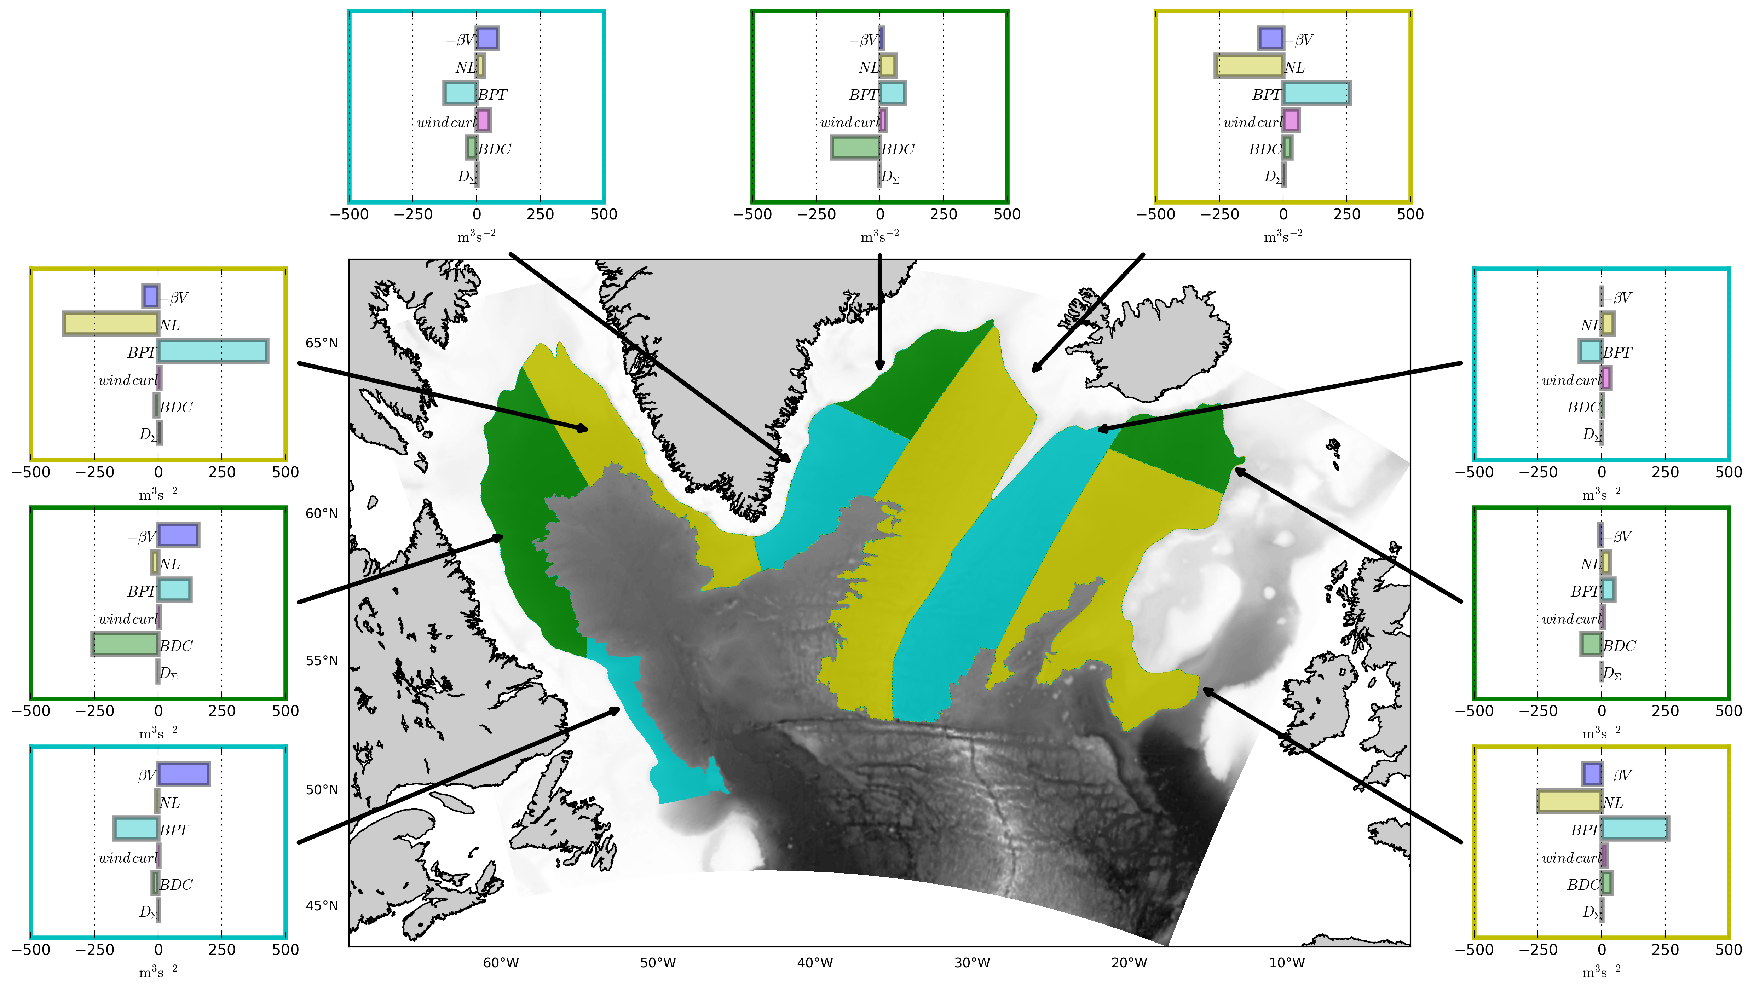
\includegraphics[width=15cm]{../fig_os/f11.pdf}
\caption{Barotropic vorticity balance integrated over different parts of the gyre along the slope}
\label{f11}
\end{figure*}

The barotropic vorticity balance in the western boundary areas (cyan in Fig. \ref{f11}) is close to the typical equilibrium of Western Boundary Currents (WBC) \citep{schoonover2016,gula2015} with an equilibrium between the planetary vorticity and the BPT. For the WLS, the deviation from WBC dynamics is small and is related to a bottom drag signal. We excluded the Southern part near Flemish Cap (48$^{\circ}$ N, 46$^{\circ}$ W) (not shown) where the dynamics is driven by a positive input of planetary vorticity and BPT balanced by the NL term. The case of the ERR is slightly different with  no net meridional transport in this area. The main input of vorticity is provided by the NL term, which is related to inertial effects from the current following the Iceland Shelf. In this area the input of positive vorticity is mainly balanced by topography and the drag corresponding to a local dissipation of vorticity. From this we can infer that western boundary areas do not provide cyclonic vorticity to the gyre interior.

Three regions (green in Fig. \ref{f11}) have in common a dominant contribution from the bottom drag. Vertical sections of the mean along-stream current (Fig. \ref{f12} (a),(c),(e)) in these areas reveal strong intensified bottom current (especially near the Iceland shelf and the Denmark Strait). In comparison, WBCs have a more surface intensified structure with reduced amplitudes near the bottom (Fig. \ref{f12} (b),(d),(f)). In Fig. \ref{f12}, vorticity balances are indicated. They differ from Fig. \ref{f11} because the integration is restricted to the boundary current, excluding recirculations. In Fig. \ref{f12} (a),(c),(e) the BPT amplitudes are reduced (and even change sign) compared to Fig. \ref{f11}. This reflects the sensitivity of the vorticity balance on the location of the boundary on the continental slope. The -3~Sv contour used in Fig. \ref{f11} does not coincide everywhere with the top of the continental slope used in Fig. \ref{f12}. 

The dynamics in the extension of the Denmark Strait and Iceland Scotland overflows is a balance between the NL term and BDC, while in the Northwestern Labrador sea, the BDC balances the $\beta$-effect. As the BDC is the main sink of vorticity and only acts locally, no advection of positive vorticity toward the inside of the gyre can come from these locations.

\begin{figure*}[t]
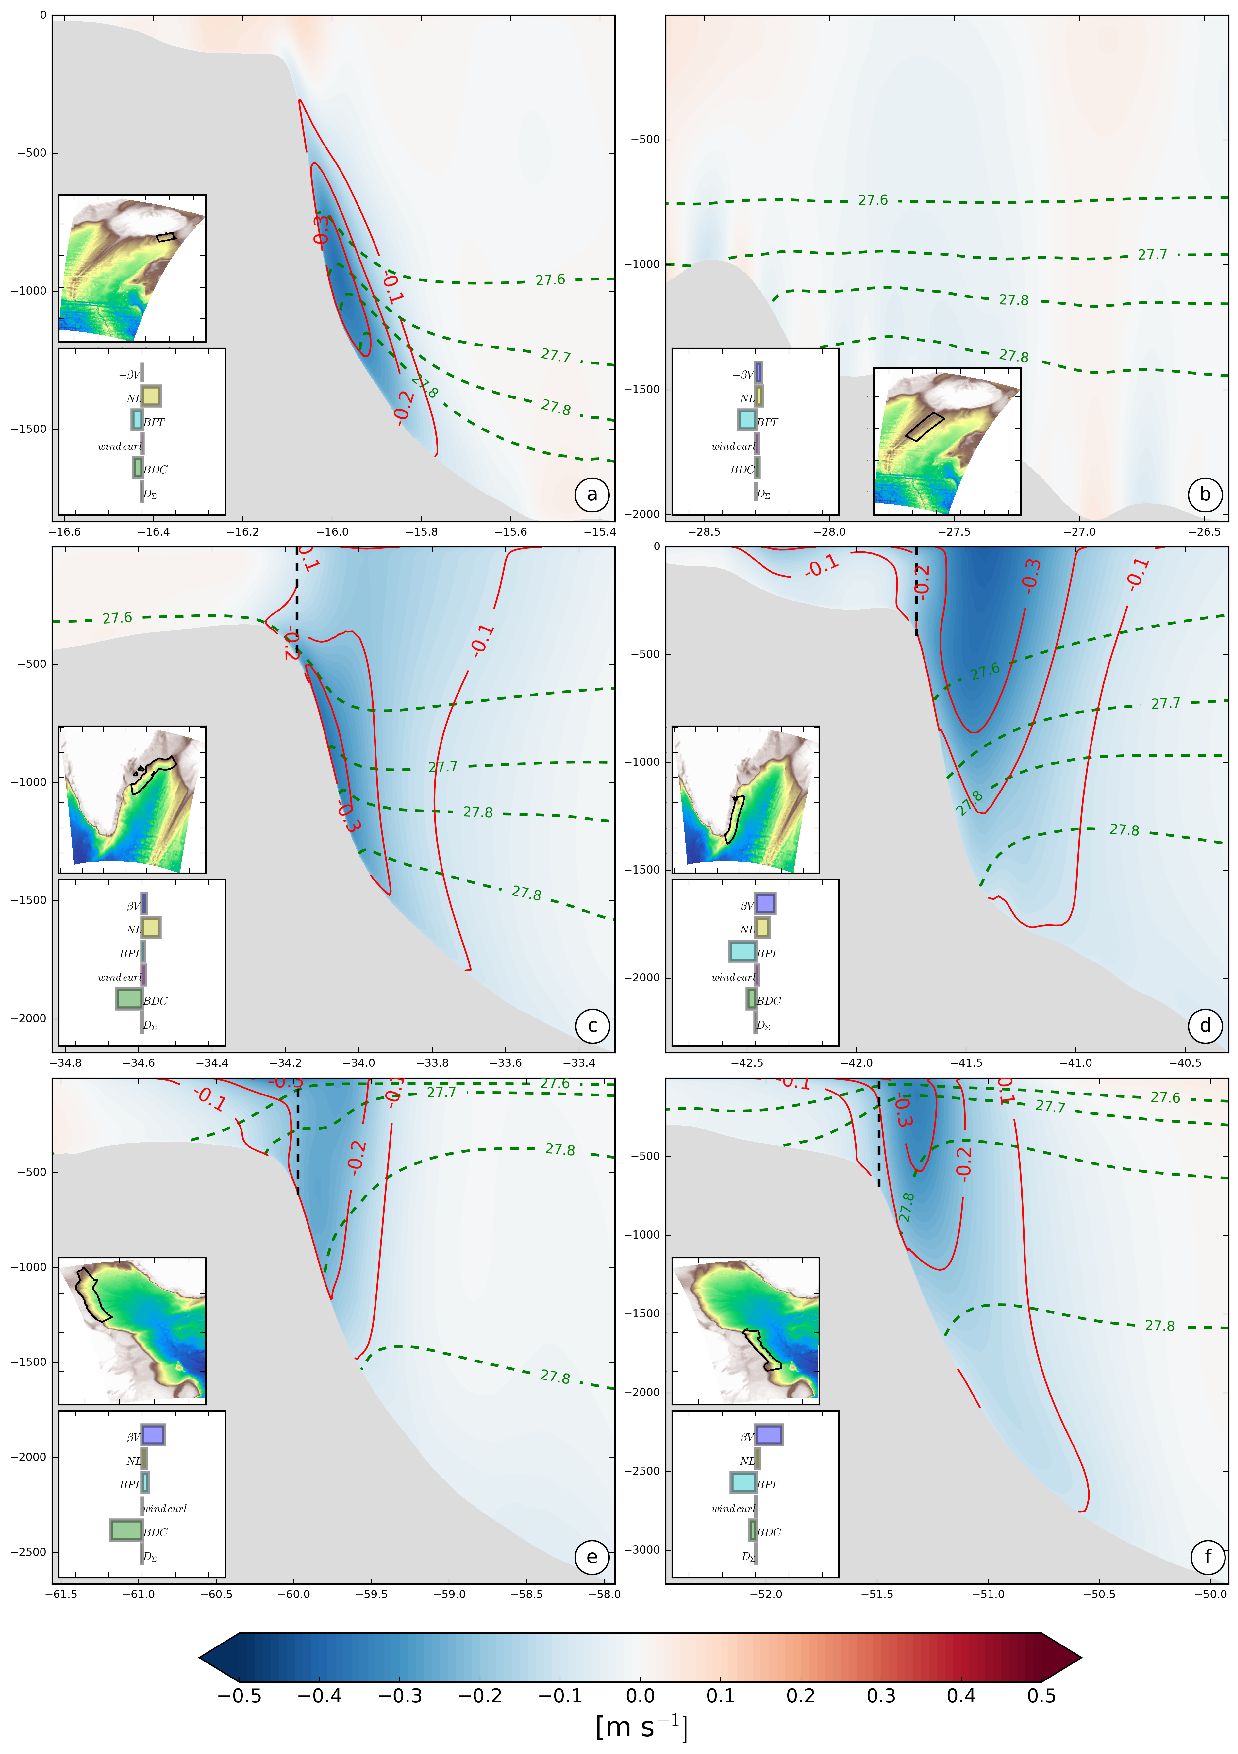
\includegraphics[width=12cm]{../fig_os/f12.pdf}
\caption{Vertical section of the mean along-stream current near Iceland shelf (a), Eastern Reykjanes Ridge (b), Denmark Strait (c), Eastern Greenland (d), Northern Labrador Current (e), and Southern Labrador Current (f). Red solid lines and green dashed lines are velocity and surface referenced potential density contours contours, respectively, while the black dashed line is the limit of integration near the shelf. The black contour on the topography map represents the area on which barotropic vorticity terms are integrated}
\label{f12}
\end{figure*} 


In Eastern boundary regions (yellow in Figure \ref{f12}), most of the cyclonic vorticity is provided by flow-topography interactions through the BPT and is balanced by the NL term. These regions are located where a strong eddy activity is observed (Figure \ref{f05}), which might be responsible for the high amplitude of the NL term. This negative NL signal implies an export of positive vorticity toward either the shelf or the gyre interior. 


\section{Characterisation of the nonlinear term}

The NL term is locally important and balances the bottom pressure torque at small scales (Fig. \ref{f06}). When integrated over the gyre it plays a role in exporting cyclonic vorticity from the boundary toward the interior of the gyre. The NL term is however quite difficult to interpret as  many processes are hidden inside the vertical and time integrals. 

By decomposing the velocity in a barotropic and baroclinic part ($u = \overline{u} + u'$) the NL advection term can be written as:
\begin{equation}
A_{\Sigma}(u,v)=\underbrace{A(\overline{u},\overline{v})}_{A^{bt}_{\Sigma}}+\underbrace{A(u',v')}_{A^{bc}_{\Sigma}}
\end{equation}

where the barotropic part can be written as $A(\overline{u},\overline{v})= \overline{u}\Omega _x +\overline{v}\Omega _y$ which is the advection of the barotropic vorticity by the barotropic flow.  

We show these terms integrated over the slope area and interior (same as Fig. \ref{f10}) in Fig. \ref{f13}. Over the slope area, both terms are negative and contribute to export cyclonic vorticity. The barotropic part is much larger than its baroclinic counterpart and export most of the vorticity, as can be expected from the barotropic structure of the currents over the slope. In the interior, both terms are positive, corresponding to an input of cyclonic vorticity for the interior (Fig. \ref{f13}), but the NL term is evenly divided between its barotropic and baroclinic contributions. The North West corner provides about half of this baroclinic NL input, while the remaining part comes mostly from the South-Eastern boundary. The exchange of barotropic vorticity is only due to the barotropic NL term between the slope region and the interior.

\begin{figure*}[t]
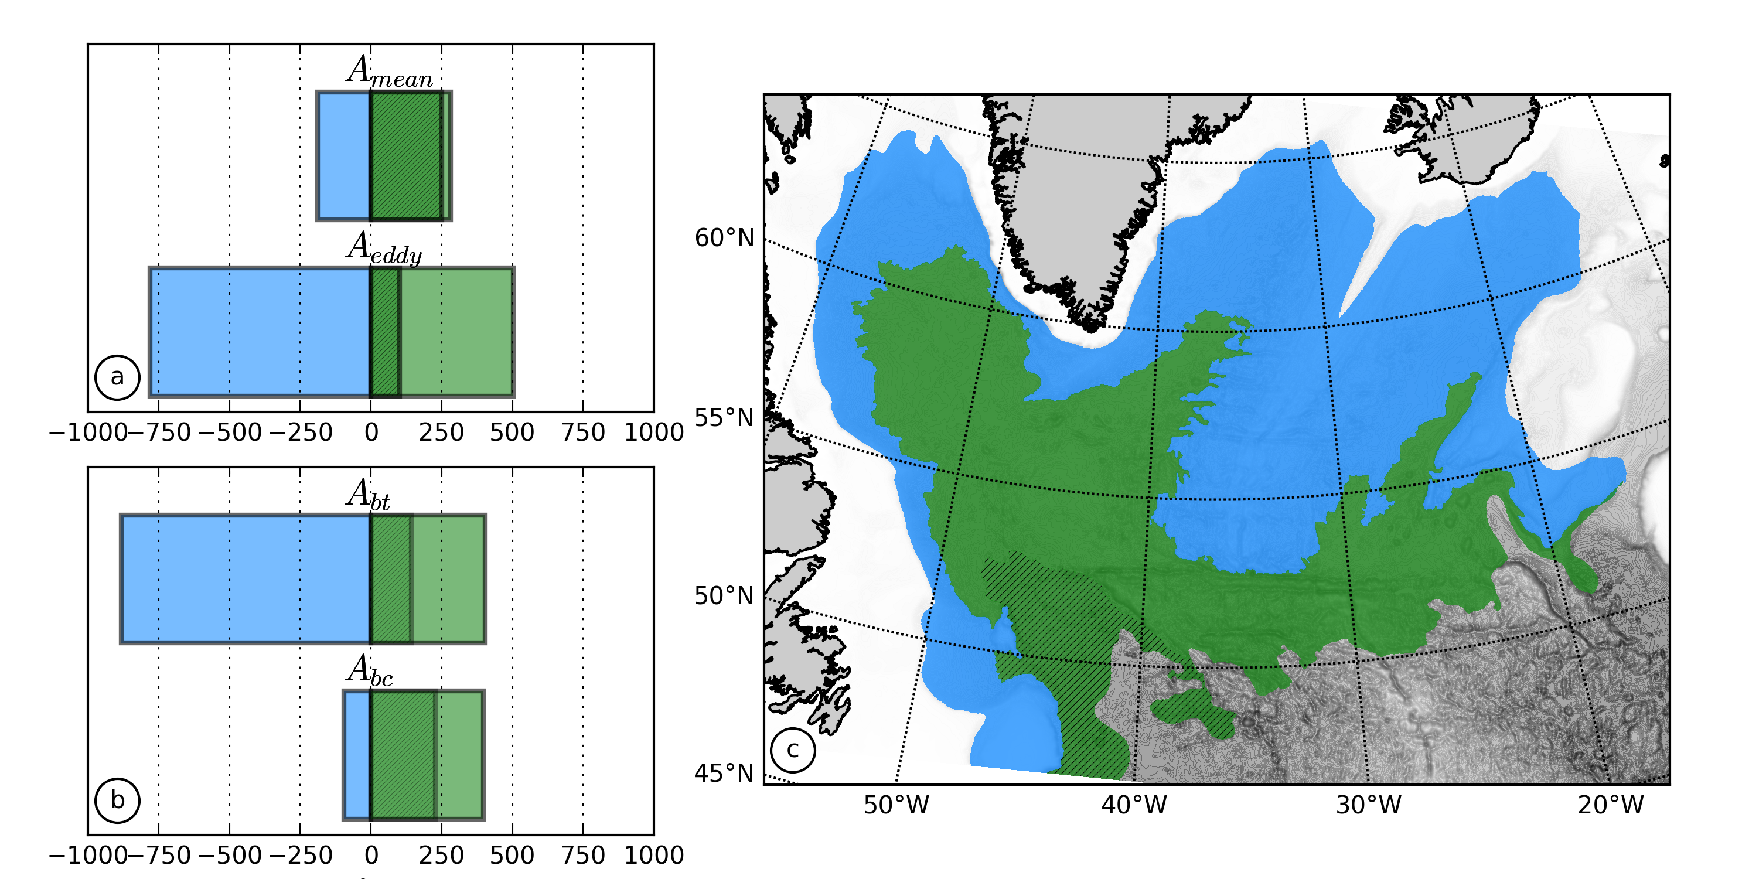
\includegraphics[width=14cm]{../fig_os/f13.pdf}
\caption{Integration of the Non linear term in the slope (c,blue) and interior area (c,green) for the mean-eddy decomposition (a)and the barotropic-baroclinic decomposition (b). The hatches are the contribution from the North Western Corner .}
\label{f13}
\end{figure*} 

It is also possible to decompose the NL term into a time mean and eddy part by writing $u = \langle u \rangle + u^*$ where $\langle \bullet\rangle$ is the time average and the star denotes the fluctuation part. By putting this in the non linear operator $A_{\Sigma}$ we have:
\begin{equation}
A_{\Sigma}(u,v)=\underbrace{A_{\Sigma}(\langle u \rangle, \langle v \rangle)}_{A_{\Sigma}^{mean}} + \underbrace{A_{\Sigma}(u^*,v^*)}_{A_{\Sigma}^{eddy}} +\underbrace{\langle  2\frac{\partial ^2 \overline{\langle v \rangle v^*} -\overline{\langle u \rangle u^*}}{\partial xy} +\frac{\partial ^2 \overline{\langle u \rangle v^*} + \overline{\langle v \rangle u^*}}{\partial xx} - \frac{\partial ^2 \overline{\langle u \rangle v^*} +\overline{ \langle v \rangle u^*}}{\partial yy}\rangle}_{\varepsilon}
\end{equation}
The $\varepsilon$ part is the residue of the cross product and its value is negligible compared to both the mean and eddy parts. 

When integrated over the slope area (Fig. \ref{f13}), the eddy component dominates over the mean one. In the interior area, the supply of barotropic vorticity is also mainly due to the eddy component but the mean component contributes about a third of the total. Almost all of this mean signal is coming from the North West corner, consistent with \citet{wang2017}, while the eddy part is dominant over the rest of the interior. 

We can identify several processes providing cyclonic barotropic vorticity to the subpolar gyre. The most important is the eddy contribution coming from the boundary area that is associated with a barotropic contribution. Barotropic vorticity is also provided through a mean-baroclinic signal coming from the NWC. In comparison, in the lower resolution simulation (not shown) most of the vorticity is advected inside the gyre by mean-barotropic processes but the amplitude of the NL term is cut by half.


\conclusions[Summary and Conclusions]
We have studied the dynamics of the North Atlantic Subpolar gyre in a numerical model with, for the first time, terrain following coordinates and a mesoscale-resolving resolution ($\Delta x \approx 2$ km). The combination of the high resolution with $\sigma$-levels allows us to better resolve the effects of the mesoscale turbulence and of the complex bottom topography. The representation of the mean currents and their variability is improved compared to previous simulations with coarser resolution. In particular, the simulations produce realistic levels of mesoscale turbulence at the surface and in the interior, as seen from comparisons of eddy potential and kinetic energy with observations from Argo floats and surface drifters.

The role of the topography is essential in the SPG. This impact is reflected in the barotropic vorticity balance of the gyre through the Bottom Pressure Torque. The Bottom Pressure Torque is sometimes interpreted as the effect of the vortex stretching due to the bottom flow over topography, as expected for a predominantly geostrophic flow. However, we show here that the ageostrophic effects, in particular due to the viscous bottom drag, are predominant at the bottom and the BPT cannot be estimated from the bottom vertical velocity. 

Barotropic vorticity balances are opposite in the shelf region compared to the interior of the gyre. The main balance in the shelf region is between a negative bottom pressure torque and a positive bottom drag, which is typical of a buoyancy driven current. Inside the gyre, the inputs of positive vorticity from the BPT and the wind curl, are balanced by the bottom drag curl. The important role played by the bottom drag and the weak role played by the viscous torque, compared to other models, is related to the choice of $\sigma$-level coordinates and high horizontal resolution. 

The bottom pressure torque has a large amplitude where boundary currents flow along the steep continental slope. It is the main term  balancing the meridional transport of water in western  boundary currents, except for some regions with dense water overflows where the bottom drag curl can become predominant. On the eastern (northward flowing) boundary currents, the strong input of positive vorticity by the bottom pressure torque is balanced by  the non linear term. The nonlinearities, which are essentially due to the eddying activity, allow advection of the positive vorticity from the boundary toward the interior of the gyre. The North Western Corner is also instrumental in feeding positive vorticity to the gyre interior through its southern boundary, mostly through time-mean baroclinic fluxes.

The nonlinear term is the main forcing for the interior part of the gyre, overcoming the effects of the wind curl and bottom pressure torque. This is putting forward the failure of the classical Sverdrup balance or even of a topographic Sverdrup balance in the interior of the Subpolar gyre, and emphasizing the importance of the inertial effects to obtain a more realistic Subpolar gyre circulation.


%% The following commands are for the statements about the availability of data sets and/or software code corresponding to the manuscript.
%% It is strongly recommended to make use of these sections in case data sets and/or software code have been part of your research the article is based on.

%\codeavailability{TEXT} %% use this section when having only software code available
\dataavailability{The datasets ANDRO and NOAA are respectively available online at \url{https://www.umr-lops.fr/Donnees/ANDRO} and \url{https://www.aoml.noaa.gov/phod/gdp/interpolated/data/subset.php}.  } %% use this section when having only data sets available
%\codedataavailability{TEXT} %% use this section when having data sets and software code available
%\sampleavailability{TEXT} %% use this section when having geoscientific samples available
%\videosupplement{TEXT} %% use this section when having video supplements available

%\appendix
%\section{}    %% Appendix A
%\subsection{}     %% Appendix A1, A2, etc.

\noappendix       %% use this to mark the end of the appendix section

%% Regarding figures and tables in appendices, the following two options are possible depending on your general handling of figures and tables in the manuscript environment:

%% Option 1: If you sorted all figures and tables into the sections of the text, please also sort the appendix figures and appendix tables into the respective appendix sections.
%% They will be correctly named automatically.
%% Option 2: If you put all figures after the reference list, please insert appendix tables and figures after the normal tables and figures.
%% To rename them correctly to A1, A2, etc., please add the following commands in front of them:
%\appendixfigures  %% needs to be added in front of appendix figures
%\appendixtables   %% needs to be added in front of appendix tables

%% Please add \clearpage between each table and/or figure. Further guidelines on figures and tables can be found below.



\authorcontribution{MLC designed the setup and carried out the experiment. MLC and JG analysed the output of the simulation. All authors participated in the writing and editing of the article.} %% this section is mandatory

\competinginterests{The authors declare that they have no conflict of interest.} %% this section is mandatory even if you declare that no competing interests are present

%\disclaimer{TEXT} %% optional section

\begin{acknowledgements}
M Le Corre is supported by UBO and Région Bretagne through ISblue, Interdisciplinary graduate school for the blue planet (ANR-17-EURE-0015) and co-funded by a grant from the French government under the program "Investissements d'Avenir". JG  is supported by UBO and AM Treguier by CNRS. Simulations were performed using HPC resources from GENCI-TGCC (grant 2018-A0050107638) and from DATARMOR of "Pôle de Calcul Intensif pour la Mer" at Ifremer, Brest, France. Model outputs are available upon request. We are grateful for comments provided by two anonymous referees that helped to improve the paper.

\end{acknowledgements}




%% REFERENCES

%% The reference list is compiled as follows:

%\begin{thebibliography}{}
\bibliographystyle{copernicus}
\bibliography{vort_240419}
%\end{thebibliography}
%\bibitem[AUTHOR(YEAR)]{LABEL1}
%REFERENCE 1
%\bibitem[AUTHOR(YEAR)]{LABEL2}
%REFERENCE 2



%% Since the Copernicus LaTeX package includes the BibTeX style file copernicus.bst,
%% authors experienced with BibTeX only have to include the following two lines:
%%
%% \bibliographystyle{copernicus}
%% \bibliography{example.bib}
%%
%% URLs and DOIs can be entered in your BibTeX file as:
%%
%% URL = {http://www.xyz.org/~jones/idx_g.htm}
%% DOI = {10.5194/xyz}


%% LITERATURE CITATIONS
%%
%% command                        & example result
%% \citet{jones90}|               & Jones et al. (1990)
%% \citep{jones90}|               & (Jones et al., 1990)
%% \citep{jones90,jones93}|       & (Jones et al., 1990, 1993)
%% \citep[p.~32]{jones90}|        & (Jones et al., 1990, p.~32)
%% \citep[e.g.,][]{jones90}|      & (e.g., Jones et al., 1990)
%% \citep[e.g.,][p.~32]{jones90}| & (e.g., Jones et al., 1990, p.~32)
%% \citeauthor{jones90}|          & Jones et al.
%% \citeyear{jones90}|            & 1990



%% FIGURES

%% When figures and tables are placed at the end of the MS (article in one-column style), please add \clearpage
%% between bibliography and first table and/or figure as well as between each table and/or figure.

%% ONE-COLUMN FIGURES

%%f







%\begin{figure}[t]
%\includegraphics[width=8.3cm]{FILE NAME}
%\caption{TEXT}
%\end{figure}
%
%%% TWO-COLUMN FIGURES
%
%%f
%\begin{figure*}[t]
%\includegraphics[width=12cm]{FILE NAME}
%\caption{TEXT}
%\end{figure*}
%
%
%%% TABLES
%%%
%%% The different columns must be seperated with a & command and should
%%% end with \\ to identify the column brake.
%
%%% ONE-COLUMN TABLE
%
%%t
%\begin{table}[t]
%\caption{TEXT}
%\begin{tabular}{column = lcr}
%\tophline
%
%\middlehline
%
%\bottomhline
%\end{tabular}
%\belowtable{} % Table Footnotes
%\end{table}
%
%%% TWO-COLUMN TABLE
%
%%t
%\begin{table*}[t]
%\caption{TEXT}
%\begin{tabular}{column = lcr}
%\tophline
%
%\middlehline
%
%\bottomhline
%\end{tabular}
%\belowtable{} % Table Footnotes
%\end{table*}
%
%%% LANDSCAPE TABLE
%
%%t
%\begin{sidewaystable*}[t]
%\caption{TEXT}
%\begin{tabular}{column = lcr}
%\tophline
%
%\middlehline
%
%\bottomhline
%\end{tabular}
%\belowtable{} % Table Footnotes
%\end{sidewaystable*}
%
%
%%% MATHEMATICAL EXPRESSIONS
%
%%% All papers typeset by Copernicus Publications follow the math typesetting regulations
%%% given by the IUPAC Green Book (IUPAC: Quantities, Units and Symbols in Physical Chemistry,
%%% 2nd Edn., Blackwell Science, available at: http://old.iupac.org/publications/books/gbook/green_book_2ed.pdf, 1993).
%%%
%%% Physical quantities/variables are typeset in italic font (t for time, T for Temperature)
%%% Indices which are not defined are typeset in italic font (x, y, z, a, b, c)
%%% Items/objects which are defined are typeset in roman font (Car A, Car B)
%%% Descriptions/specifications which are defined by itself are typeset in roman font (abs, rel, ref, tot, net, ice)
%%% Abbreviations from 2 letters are typeset in roman font (RH, LAI)
%%% Vectors are identified in bold italic font using \vec{x}
%%% Matrices are identified in bold roman font
%%% Multiplication signs are typeset using the LaTeX commands \times (for vector products, grids, and exponential notations) or \cdot
%%% The character * should not be applied as mutliplication sign
%
%
%%% EQUATIONS
%
%%% Single-row equation
%
%\begin{equation}
%
%\end{equation}
%
%%% Multiline equation
%
%\begin{align}
%& 3 + 5 = 8\\
%& 3 + 5 = 8\\
%& 3 + 5 = 8
%\end{align}
%
%
%%% MATRICES
%
%\begin{matrix}
%x & y & z\\
%x & y & z\\
%x & y & z\\
%\end{matrix}
%
%
%%% ALGORITHM
%
%\begin{algorithm}
%\caption{...}
%\label{a1}
%\begin{algorithmic}
%...
%\end{algorithmic}
%\end{algorithm}
%
%
%%% CHEMICAL FORMULAS AND REACTIONS
%
%%% For formulas embedded in the text, please use \chem{}
%
%%% The reaction environment creates labels including the letter R, i.e. (R1), (R2), etc.
%
%\begin{reaction}
%%% \rightarrow should be used for normal (one-way) chemical reactions
%%% \rightleftharpoons should be used for equilibria
%%% \leftrightarrow should be used for resonance structures
%\end{reaction}
%
%
%%% PHYSICAL UNITS
%%%
%%% Please use \unit{} and apply the exponential notation


\end{document}